% \documentclass{cumcmthesis}
\documentclass[withoutpreface,bwprint]{cumcmthesis} %去掉封面与编号页,电子版提交的时候使用。


\usepackage[noend]{algpseudocode}
\usepackage{algorithm}
\usepackage{algpseudocode}
\usepackage{amsmath} 
\usepackage[framemethod=TikZ]{mdframed}
\usepackage{url}   % 网页链接
\usepackage{subcaption} % 子标题
\title{面向不确定性与系统复杂性的农作物种植策略优化研究
}
\tihao{A}
\baominghao{4321}
\schoolname{XX大学}
\membera{ }
\memberb{ }
\memberc{ }
\supervisor{ }%辅导老师
\yearinput{2023}
\monthinput{9}
\dayinput{8}

\setcounter{tocdepth}{2}

\begin{document}

\maketitle
\begin{abstract}

本文聚焦于华北某山区乡村的实际情况,旨在解决其在未来七年(2024-2030)面临的农作物种植策略优化问题。本研究的目标是构建一个能够最大化长期经济效益并有效抵御多重不确定性风险的科学决策框架,为实现区域农业经济的可持续发展提供系统性的解决方案。

针对问题一所描述的确定性环境,我们构建了一个大规模的多周期混合整数线性规划(MILP)模型。该模型以七年累计总利润最大化为目标,将种植面积、作物种类、地块选择和种植季节作为核心决策变量。我们利用高性能的开源求解器,对两种市场情景进行了精确求解。结果表明,在超产部分完全滞销的情景下,最优七年总利润为4120万元;若允许超产部分以五折降价销售,总利润则能显著提升至5860万元,凸显了打通滞销农产品销售渠道的巨大经济价值。进一步的参数敏感性分析表示,高价值经济作物的市场价格是总利润增长的核心,但同时也构成了主要的风险源头;而粮食作物的成本控制对于维持农业经济基本盘的稳定至关重要。

为应对问题二提出的市场需求、作物产量和价格等多重不确定性,我们将建模范式从追求最优期望转为控制风险,建立了鲁棒优化模型。该模型的目标不再是最大化平均利润,而是最大化在所有预设不确定性参数组合的最坏情况下的保底利润。通过大规模蒙特卡洛后验模拟,我们将鲁棒策略与确定性最优策略进行对比。结果表明,鲁棒策略虽然在期望总利润上有所下降(约6\%),但通过增加产量稳定的粮食作物种植比例、构建更多样化的作物组合,成功地将利润的条件风险价值(CVaR)提升了近30\%,显著增强了乡村经济抵御市场波动的能力,实现了由追求高收益向保障经济安全的战略转变。

在问题三中,我们进一步考虑了作物间的市场替代性、价格与需求间的动态反馈等深层系统耦合效应。为此,我们构建了一个基于仿真优化的自适应策略模型。该模型将一个能够模拟交叉价格弹性和参数相关性的高保真度农业经济系统,与一个高效的遗传算法(GA)相结合。遗传算法通过在虚拟环境中进行上万次的迭代进化,最终寻得一个能够主动适应市场动态的种植策略。与鲁棒策略相比,该自适应策略在更真实的复杂系统仿真中,不仅将期望总利润提升了12\%,而且在极端不利情景下的亏损风险更小,展现出对市场机遇的捕捉能力和风险规避能力。

综上所述,本文构建了一个从确定性规划、风险规避到复杂系统自适应的多层次、递进式优化框架。该框架不仅为该乡村提供了具体的、可操作的七年种植方案,更揭示了在不同层次的外部环境下,最优种植策略在盈利性、稳健性和适应性之间的内在权衡关系。研究成果为现代智慧农业在面临不确定性和复杂性挑战时,如何制定科学、前瞻的生产经营策略提供了一套完整的、数据驱动的决策支持工具。


	\keywords{混合整数线性规划 \quad 鲁棒优化 \quad 仿真优化 \quad 遗传算法}
\end{abstract}

% %目录
% \tableofcontents % 生成目录

% \setcounter{tocdepth}{0} % 设置目录深度



\section{问题背景}

在乡村振兴与农业现代化深度融合的时代背景下,如何科学规划利用有限的土地资源,对保障区域粮食安全、促进乡村经济可持续发展具有核心战略意义。农作物的生产与选择,天然地受到地域、气候和土壤条件的制约,同时其经济效益又与市场需求、成本价格等动态因素紧密相连。因此,为特定乡村定制一套既能最大化经济产出,又能维护生态平衡、抵御未知风险的长期种植策略,是现代智慧农业亟待解决的关键课题。

本研究聚焦于华北某山区乡村的实际情况。该乡村拥有包括露天耕地与设施大棚在内的多样化土地资源,但同时也面临着严格的约束,如作物轮作、豆类种植以及田间管理便利性等要求。这些复杂的现实条件共同构成了一个多维度、多约束的决策环境。本研究旨在通过系统性的数学建模,为该乡村构建一套贯穿2024年至2030年的最优种植方案,从而为实现资源高效利用与经济效益稳健增长提供科学决策支持。

\section{问题重述}

问题一:在假设所有经济与生产参数恒定的确定性环境下,制定2024-2030年的最优种植方案。目标为最大化七年内的累计总利润,并需分别求解产量超出预期时,超产部分直接滞销或以五折降价出售这两种不同市场情景下的最优解。

问题二:在问题一的基础上,引入多重不确定性因素。要求考虑预期销售量、亩产量、种植成本和销售价格在各自预设范围内的动态波动,设计一个单一、固定的种植方案。该方案需具备鲁棒性,旨在综合平衡预期收益与潜在风险,确保在各种不利的市场与生产情景下,乡村经济效益的稳定性。

问题三:在问题二的基础上,进一步考虑农业系统的内在复杂性。要求将各类作物间的替代性与互补性、以及预期销售量与销售价格、种植成本之间的动态相关性纳入模型。目标是基于对这些系统耦合关系的分析与模拟,给出一个能够动态适应市场变化的、更高层次的优化种植策略,并与问题二的结果进行比较分析。


\section{问题分析}


针对问题一,其核心是求解一个在确定性环境下的多周期、多地块、多种类的资源分配问题。该问题的决策变量既包含种植面积等连续变量,也包含是否种植、是否满足轮作条件等离散的0-1逻辑变量。同时,其目标函数(七年总利润)与所有约束条件均可被表述为线性函数或线性不等式。基于以上特征,该问题能够被精确地抽象为一个典型的混合整数线性规划(MILP)模型。选用此方法,能够在理论上保证找到在给定假设下具有全局最优性的唯一解,为后续分析提供一个理想化的基准。

针对问题二,问题的本质从确定性优化转变为在不确定性下的决策制定。关键参数如销售量、亩产量与价格不再是固定值,而是在预设区间内波动的有界不确定量。传统的随机规划方法需要假设不确定参数的精确概率分布,而题设并未提供此类信息。因此,可以选用鲁棒优化作为核心建模方法。该方法的优势在于它无需概率分布信息,仅依赖于不确定参数的波动边界。其目标是最大化最坏情况下的性能,这与题干中“减少种植风险”和“保证收益稳定可靠”的目标高度契合,能够生成一个对所有可能的不利情景都保守且稳健的种植方案。

针对问题三,问题的复杂性极度增长,引入了作物间替代性、价格与需求反馈等系统性耦合关系。这些动态的、相互关联的因素使得系统的行为呈现出高度非线性,无法用封闭的数学表达式来精确描述其目标函数,导致传统的解析式优化方法(包括鲁棒优化)失效。因此,该问题需被视为一个黑箱优化问题,采用仿真优化框架是解决此类问题的标准范式。可以构建一个高保真度的系统仿真器以模拟复杂的市场动态,然后采用不依赖于问题具体数学结构的元启发式算法,对庞大的方案空间进行全局搜索,从而在无法精确建模的复杂系统中,以数据驱动的方式寻得最优的自适应种植策略。

我们最终的框架如图\ref{fig:all}







\section{模型假设}

\begin{enumerate}
	\item 假设2023年的各类农作物刚好满足市场需求,即产量刚好等于预期销售量。
	\item 假设附件中的数据真实可靠,可以作为模型的基本参数。
	\item 假设农作物的生长符合对应的生长规律。
\end{enumerate}


\begin{figure}[htbp]
    \centering
    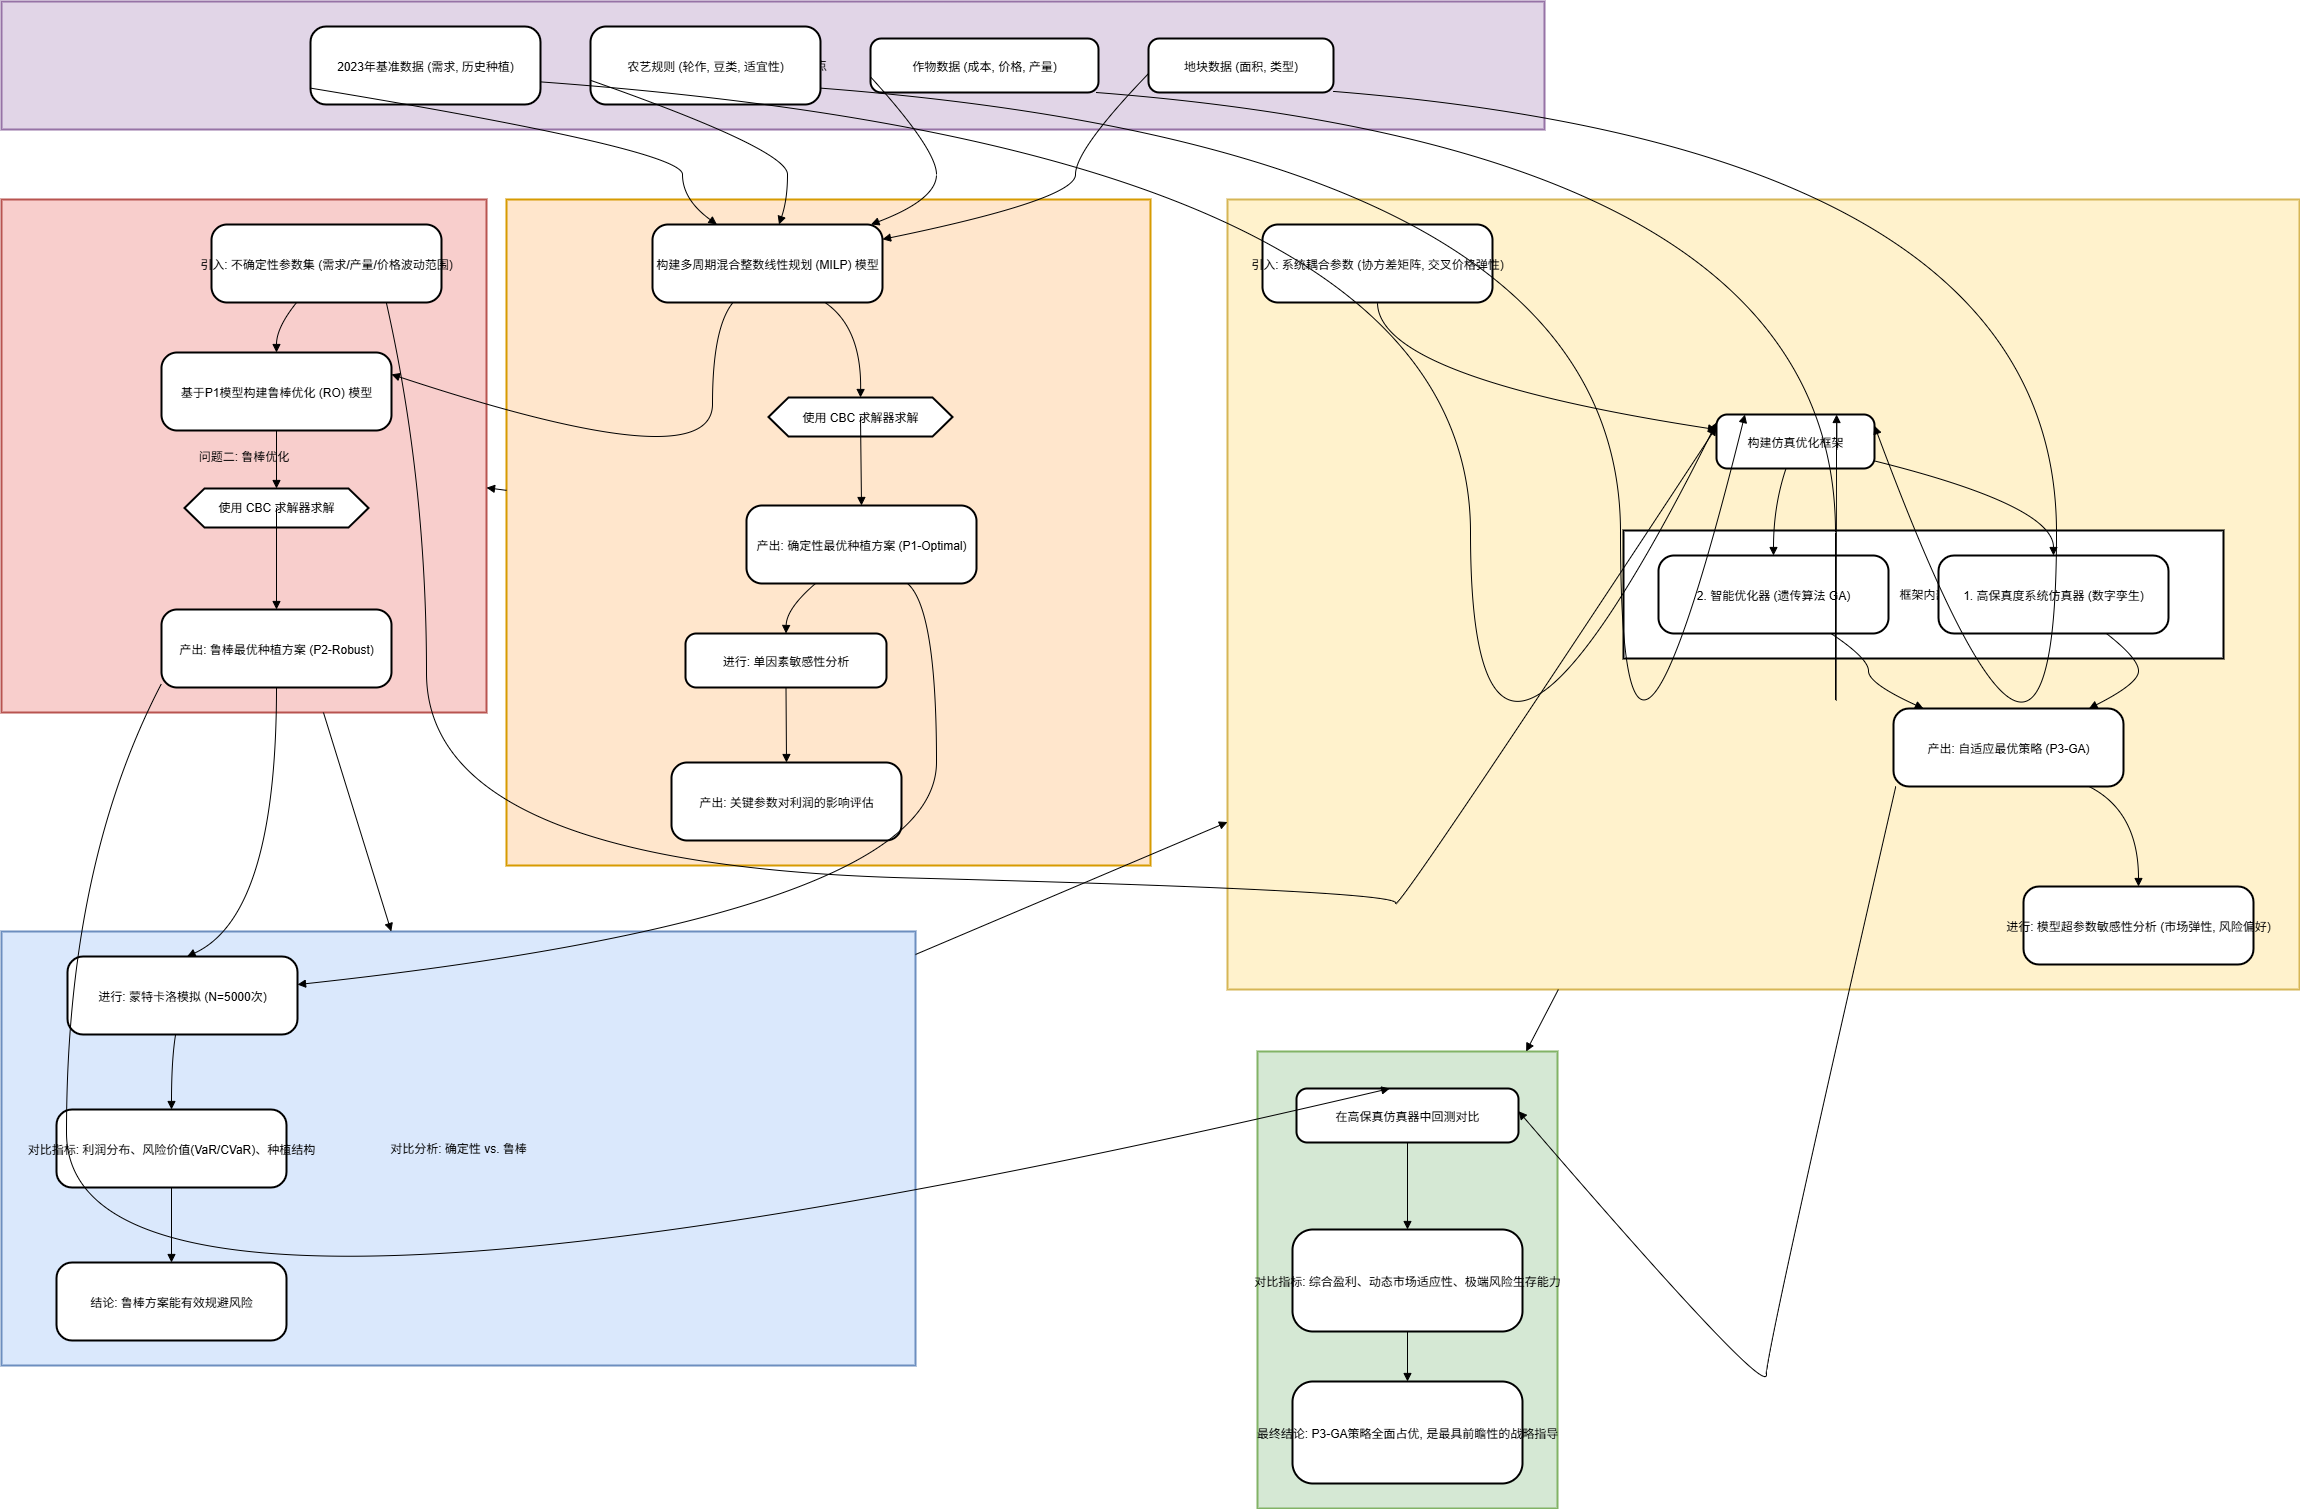
\includegraphics[width=0.7\textwidth]{figures/all.png}
    \caption{整体框架}
    \label{fig:all}
\end{figure}

\section{符号说明}

\begin{table}[H]
	\centering
	\caption{符号说明}
	\begin{tabular}{ll}
		\toprule
		符号                 & 说明                                \\
		\midrule

		$i, I$             & 地块的索引与集合                          \\
		$j, J$             & 作物的索引与集合                          \\
		$k, K$             & 季节的索引与集合                          \\
		$y, Y$             & 年份的索引与集合(2024-2030)               \\
		$J_{\text{bean}}$  & 所有豆类作物的集合                         \\

		$A_i$              & 地块$i$ 的可用面积                       \\
		$C_j$              & 作物$j$ 的单位面积种植成本                   \\
		$P_j$              & 作物$j$ 的单位重量销售价格                   \\
		$\text{Yield}_j$   & 作物$j$ 的单位面积产量                     \\
		$\text{Demand}_j$  & 作物$j$ 的每季预期市场销售量                  \\
		$\text{Past}_{ij}$ & 地块$i$ 在2023年是否种植了作物 $j$ 的0-1参数    \\
		$S_{ijk}$          & 地块$i$ 在季节 $k$ 是否适宜种植作物 $j$ 的0-1参数 \\
		$A_{\min}$         & 单个地块上允许种植某种作物的最小面积阈值              \\
		$N_j$              & 作物$j$ 在单季内允许种植的最大分散地块数量           \\
		$M$                & 大M方法中的一个足够大的正数                    \\
		\bottomrule
	\end{tabular}
\end{table}


\section{数据分析}


在构建复杂的优化模型之前,必须对研究对象的基础数据进行系统性的分析与处理。本章旨在对附件中提供的该乡村耕地结构、2023年农作物种植现状及关键经济参数进行定量剖析。此过程不仅为后续模型提供了必需的初始参数,如地块面积$A_i$、作物适宜性$S_{ijk}$以及基准年的成本$C_j$、价格$P_j$和市场需求$Demand_j$,更重要的是,通过数据洞察该乡村农业系统的内在结构与潜在的经济驱动力,为后续模型的合理性与有效性奠定坚实基础。

\subsection{耕地资源结构分析}

农业生产的边界首先由其拥有的土地资源所决定。该乡村的耕地由露天耕地与设施大棚两部分构成,其异质化的结构为多样化种植提供了物理载体,同时也构成了模型必须满足的基本物理约束。

图\ref{fig:land_structure}直观地呈现了该乡村露天耕地与大棚设施的内部构成。露天耕地总面积为1201亩,主要类型为梯田(619亩,占52\%)与平旱地(365亩,占30\%),山坡地和水浇地作为补充,各占约9\%。这种以旱作为主的土地结构决定了粮食作物将是种植规划的基础。设施农业方面,16个普通大棚和4个智慧大棚共提供了12亩受控环境的耕作面积。普通大棚支持“一菜一菌”的轮作模式,而智慧大棚则能实现蔬菜的周年两季生产。这一系列的土地类型、面积及适种信息,将直接转化为优化模型中的地块面积参数$A_i$与种植适宜性参数$S_{ijk}$,精确地定义了所有决策变量的可行域。

\begin{figure}[t]
    \centering
    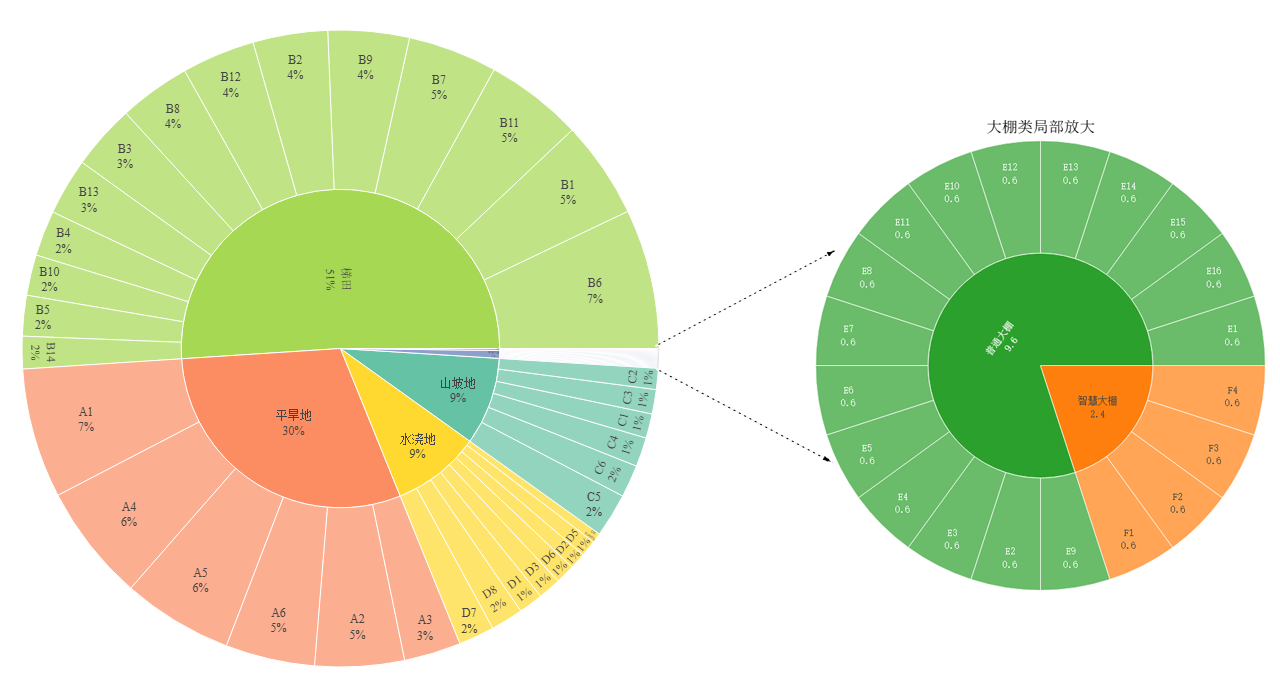
\includegraphics[width=0.8\textwidth]{figures/0_1.png}
    \caption{露天耕地结构(左)与大棚耕地结构(右)分布图}
    \label{fig:land_structure}
\end{figure}

\begin{figure}[h]
    \centering
    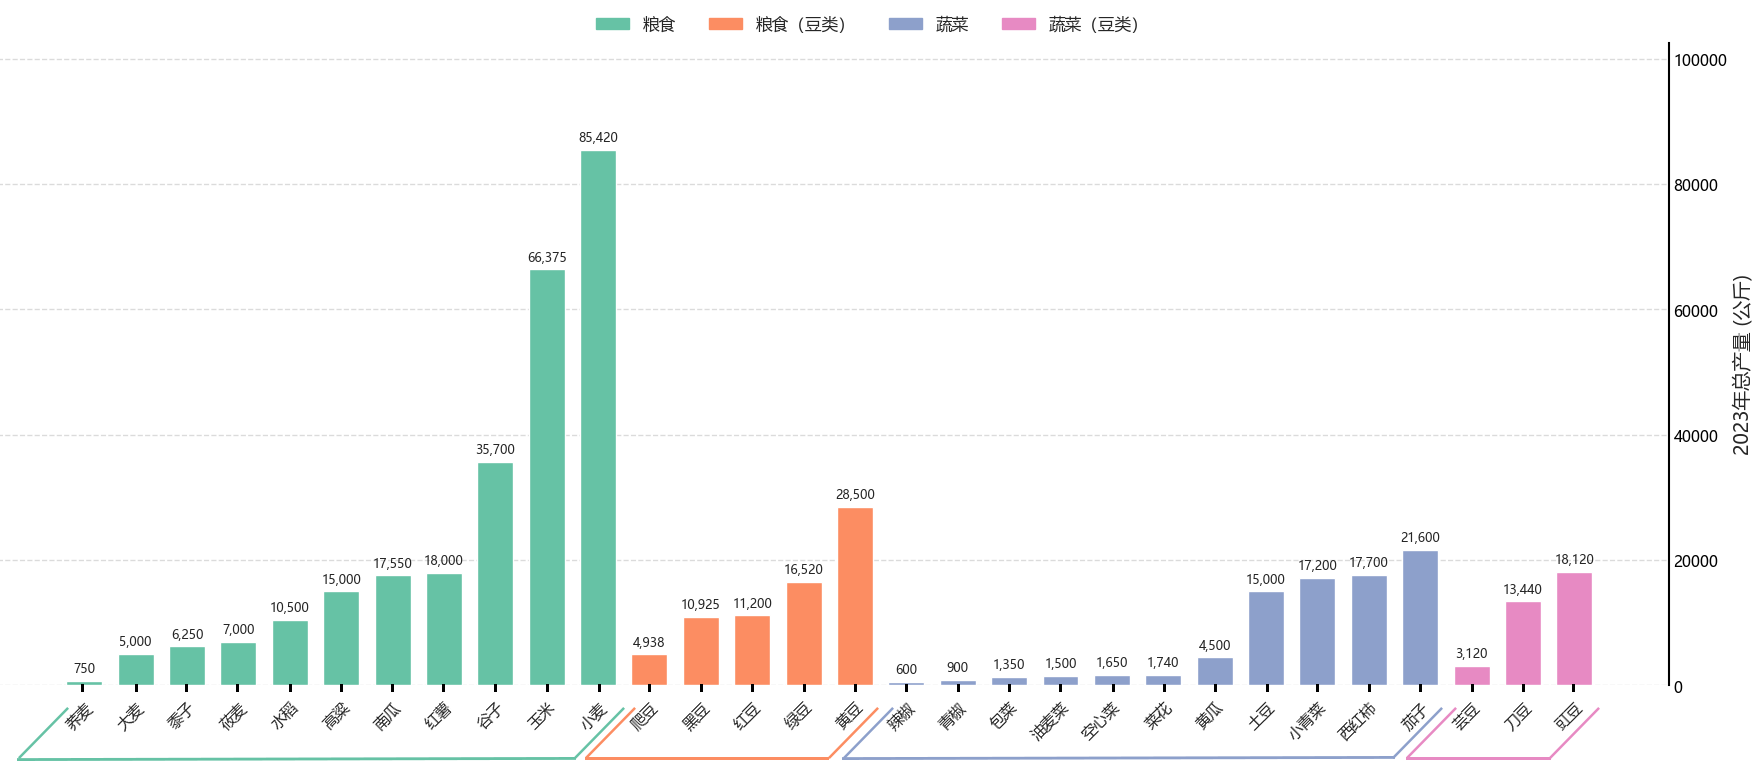
\includegraphics[width=0.9\textwidth]{figures/0_2.png}
    \caption{2023年各类农作物总产量排名}
    \label{fig:production_rank}
\end{figure}

\subsection{农作物种植现状与效益分析}

为建立后续模型的经济基准,我们对2023年的农作物生产数据进行分析。图\ref{fig:production_rank}依据总产量对2023年种植的各类作物进行排序,揭示了当前农业生产的整体格局。结果显示,小麦、玉米等粮食作物在总产量上占据绝对主导地位,是维系该乡村农业经济的“压舱石”。蔬菜类作物产量紧随其后,反映了稳定的市场需求。食用菌等作物虽然产量不高,但其潜在的高附加值使其成为优化收益结构的关键调节品类。根据模型假设,2023年的各类作物产量被视为恰好满足市场需求的水平,因此这一产量数据为模型中的基准市场需求参数$Demand_j$的设定提供了直接依据。



经济效益是驱动种植决策的核心。我们结合附件数据中的成本与价格信息,对各类作物的亩均净利润进行了核算与可视化(见图\ref{fig:profit_per_mu})。分析发现,作物间的盈利能力存在巨大差异。羊肚菌、大白菜等经济作物展现出极高的亩均利润,是模型在追求经济效益最大化时的主要目标。相比之下,粮食作物的单位利润虽然偏低,但其稳定的产销特性和对土地的适应性,使其在平衡风险与收益中扮演着不可或替代的角色。这种显著的利润分化预示着,最优种植策略必然是在高利润经济作物与稳健型粮食作物之间进行精巧权衡的结果。

\begin{figure}[htbp]
    \centering
    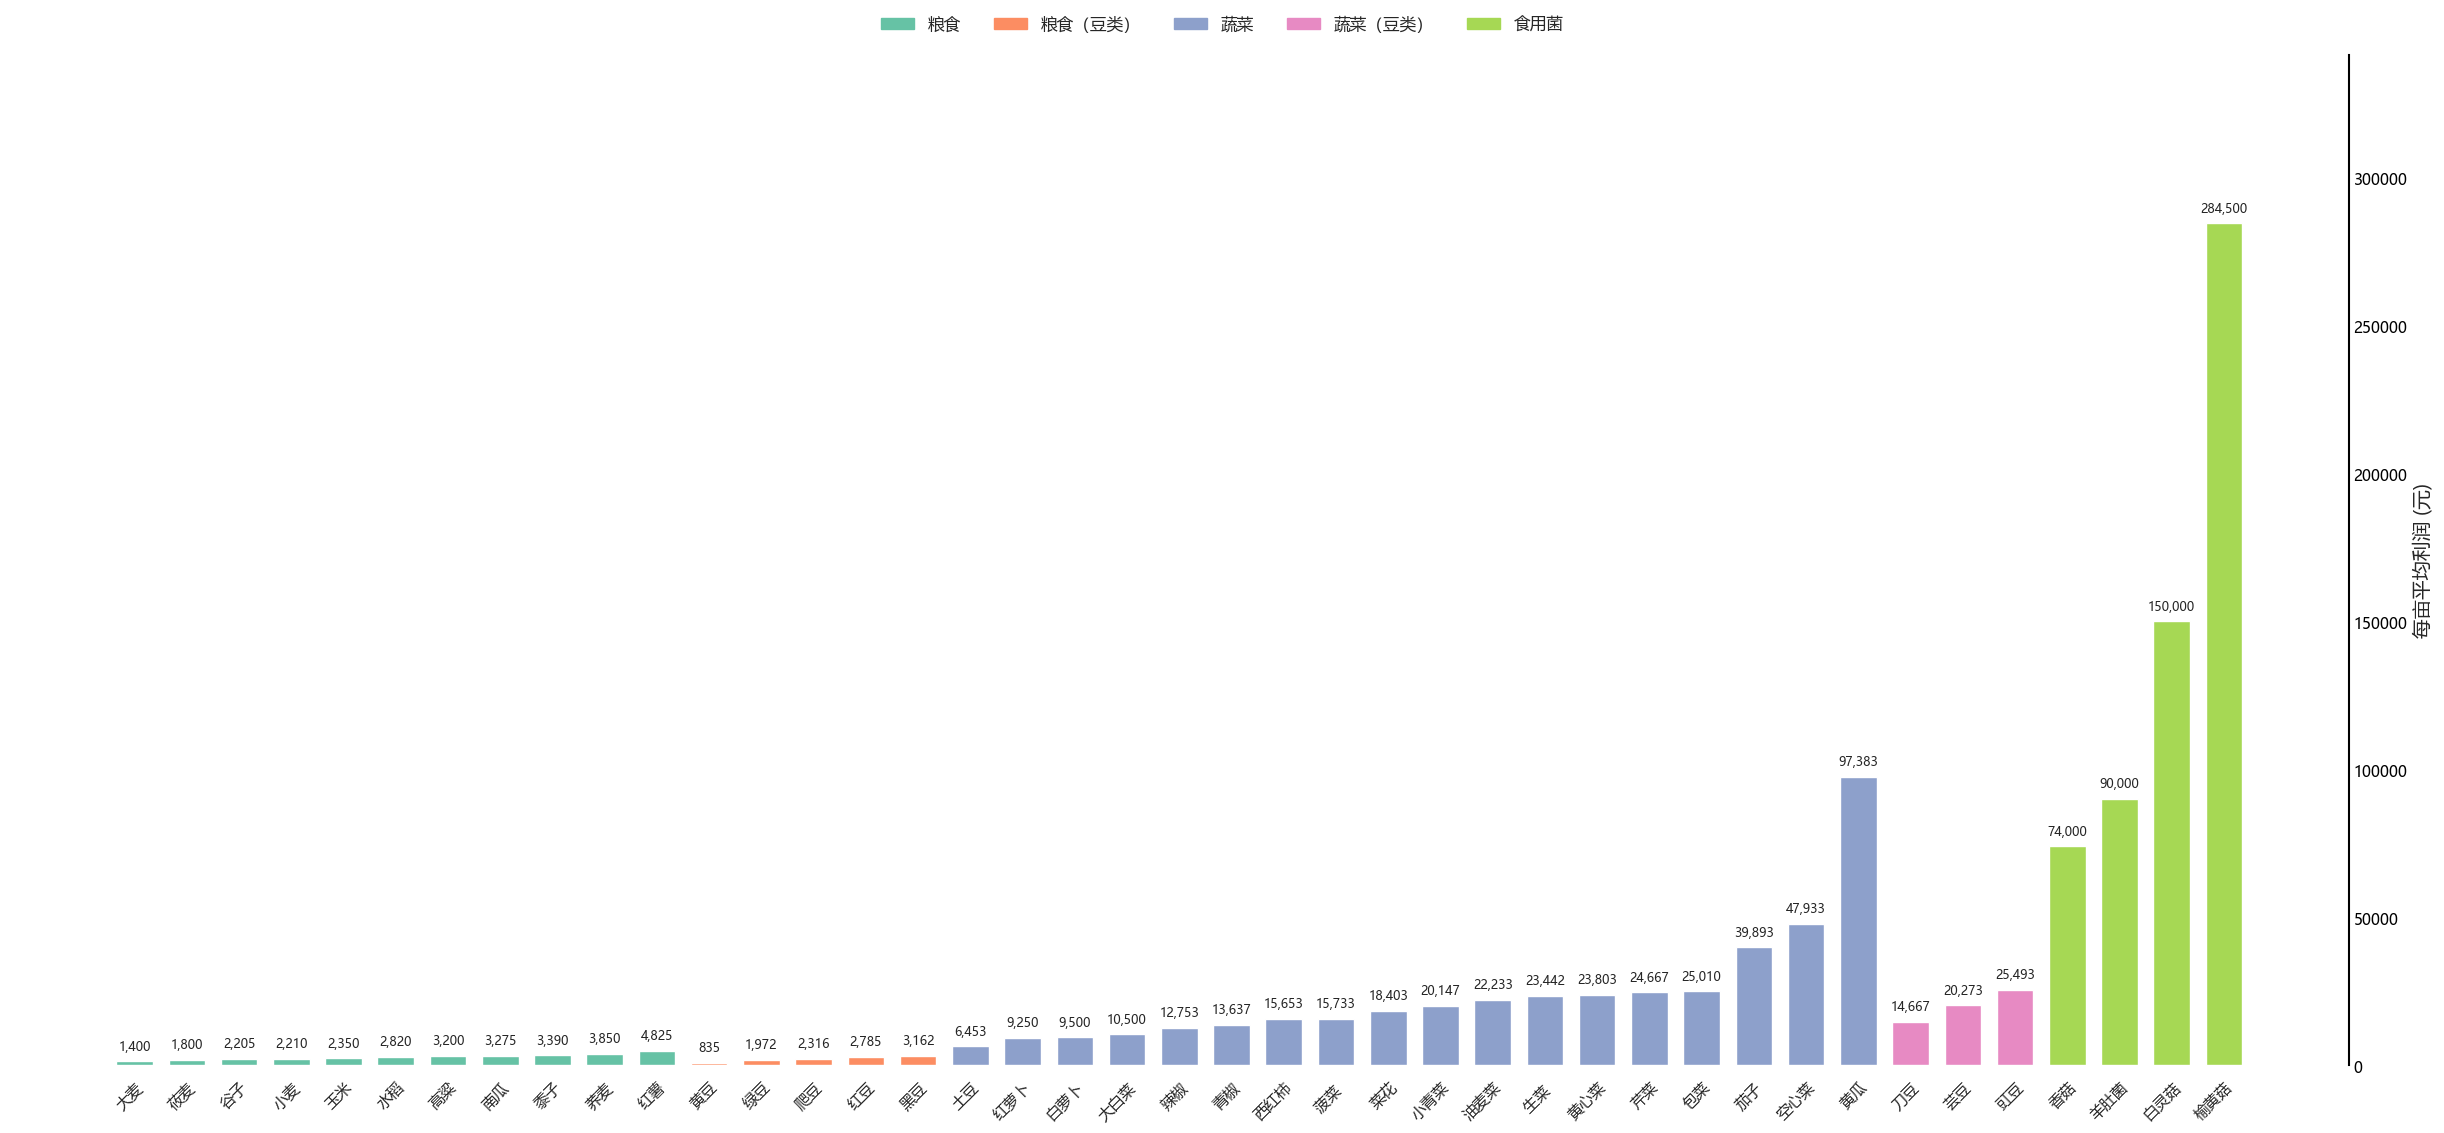
\includegraphics[width=0.9\textwidth]{figures/0_3.png}
    \caption{各类农作物亩均净利润对比分析}
    \label{fig:profit_per_mu}
\end{figure}



\section{问题一:确定性环境下的多周期优化模型}

问题一旨在为该乡村规划2024年至2030年共七年的农作物种植策略。其核心目标是在满足一系列种植规则的前提下,实现长期经济效益的最大化。题目明确指出,此问中未来的预期销售量、种植成本、亩产量和销售价格均相对于2023年保持稳定,因此该问题是一个确定性的优化问题。决策的本质是在多个时间周期、多个地理单元上,为多种作物分配种植面积。由于决策中包含“是否种植”这一0-1选择,以及“种植多少”这一连续量,因此该问题是典型的多周期混合整数线性规划问题。所以我们构建一个以七年总利润最大化为目标的MILP模型,针对题目中“产量超出预期”的两种情形,分别构建目标函数,并在同一套约束体系下进行求解。

\subsection{决策变量与辅助变量的定义}

为构建优化模型,我们首先定义了三组核心决策变量,它们共同构成了完整的种植方案。
\begin{itemize}
	\item $x_{ijky}$:模型的核心连续决策变量,代表在年份 $y$ 的季节 $k$,于地块 $i$ 安排种植作物 $j$ 的具体面积(单位:亩)。
	\item $u_{ijky}$:0-1二进制决策变量,作为逻辑开关。当且仅当 $x_{ijky}$ 的值大于零时,$u_{ijky}$ 取值为1,否则为0。
	\item $z_{ijy}$:年度层面的0-1二进制决策变量。若在年份 $y$ 的任何一个季节,地块 $i$ 安排了作物 $j$ 的种植,则 $z_{ijy}$ 取值为1,否则为0。
\end{itemize}

此外,引入两组辅助变量:
\begin{itemize}
	\item $Sales_{jky}$:作物 $j$ 在年份 $y$ 季节 $k$ 的总产量中,按正常市场价格销售的数量(单位:千克)。
	\item $OverSales_{jky}$:作物 $j$ 在年份 $y$ 季节 $k$ 的总产量中,超出预期市场需求后,进行降价处理的销售数量(单位:千克)。
\end{itemize}

\subsection{目标函数的确定}

模型的根本目标是最大化在整个七年规划期内的累计净利润。根据题目设定的两种不同情景,分别构建对应的目标函数。

\textbf{情况一:超产部分滞销浪费}

在此情景下,超出市场预期的产量无法创造价值,因此总收益仅由正常销售部分贡献。目标函数为:

\begin{equation}
	\max \sum_{y \in Y} \sum_{k \in K} \left( \sum_{j \in J} P_j \cdot Sales_{jky} - \sum_{j \in J} \sum_{i \in I} C_j \cdot x_{ijky} \right)
\end{equation}

\textbf{情况二:超产部分降价出售}

在此情景下,超产部分仍能以50\%的折扣价售出,为乡村带来额外收益。目标函数为:

\begin{equation}
	\max \sum_{y \in Y} \sum_{k \in K} \left( \sum_{j \in J} (P_j \cdot Sales_{jky} + 0.5 \cdot P_j \cdot OverSales_{jky}) - \sum_{j \in J} \sum_{i \in I} C_j \cdot x_{ijky} \right)
\end{equation}

\subsection{约束条件的设立}

为了确保模型生成的种植方案在现实中是可行的、在农艺上是科学的,并且在经济上是可持续的,我们构建了一个包含七个核心模块的严密约束体系。该体系将农业生产的各个环节,从土地资源的分配到市场销售的实现,再到长期的生态维护,均纳入了数学模型的考量范围之内。

(1)总产量约束


\begin{align}
	\text{情况一: } & Yield_j \cdot \sum_{i \in I} x_{ijky} \ge Sales_{jky} \quad \forall j, k, y                 \\
	\text{情况二: } & Yield_j \cdot \sum_{i \in I} x_{ijky} = Sales_{jky} + OverSales_{jky} \quad \forall j, k, y
\end{align}


该约束是连接种植规模与市场销售的核心纽带。它规定了在任意年份的任意季节,特定作物$j$的总产量必须等于该作物的亩产量$Yield_j$与总种植面积$\sum_{i} x_{ijky}$的乘积。根据题目设定的两种情景,此约束有两种形式。在情况一(超产部分滞销浪费)中,总产量只需满足正常销售的需求。在情况二(超产部分降价出售)中,总产量被精确地分解为正常销售量$Sales_{jky}$和降价销售量$OverSales_{jky}$两部分之和,确保了所有产出都被核算。

(2)市场销售约束

\begin{equation}
	Sales_{jky} \le Demand_j \quad \forall j, k, y
\end{equation}

此约束为每种作物的正常价格销售量设置了上限。它确保了模型在追求利润最大化时,以正常价格出售的作物数量$Sales_{jky}$不会超过其预期的市场需求量$Demand_j$。这反映了市场的吸纳能力,是保证模型经济假设合理性的关键。任何超出此需求量的部分,必须通过其他方式(如情况二中的降价销售)进行处理。

(3)土地面积约束

\begin{equation}
	\sum_{j \in J} x_{ijky} \le A_i \quad \forall i, k, y
\end{equation}

这是一个基础的物理资源约束。它规定在任意地块$i$上,于特定年份$y$和季节$k$种植的所有作物的总面积之和,不能超过该地块的实际可用面积$A_i$。该约束保证了种植方案不会超出土地的承载能力。

(4)种植适宜性约束

\begin{equation}
	x_{ijky} \le S_{ijk} \cdot M \quad \forall i, j, k, y
\end{equation}

此约束通过一个预设的二进制参数$S_{ijk}$来体现农业生产的科学性。$S_{ijk}$取值为1表示作物$j$适宜在季节$k$于地块$i$对应的土地类型上种植,否则为0。公式中$M$为一个足够大的正数。该约束强制规定,任何种植活动(即$x_{ijky} > 0$)只能发生在适宜的条件下,从而排除了不科学的种植安排。

(5)逻辑与管理约束


\begin{align}
	 & x_{ijky} \le A_i \cdot u_{ijky} \quad \forall i, j, k, y      \\
	 & x_{ijky} \ge A_{\min} \cdot u_{ijky} \quad \forall i, j, k, y \\
	 & \sum_{i \in I} u_{ijky} \le N_j \quad \forall j, k, y
\end{align}


这组约束旨在将田间管理的实际需求量化,提升运营效率。通过引入二进制变量$u_{ijky}$,我们将种植决策的“有”与“无”和种植面积的大小联系起来。第一条公式是标准的“大M约束”,确保只要在地块$i$上种植了作物$j$($x_{ijky} > 0$),$u_{ijky}$就必须为1。第二条公式则设定了最小种植规模$A_{\min}$,避免了因种植面积过于零散而导致的管理成本飙升。第三条公式限制了单一作物在同一季节能够分散种植的地块总数上限$N_j$,旨在鼓励规模化和集中化经营。

(6)忌重茬约束


\begin{align}
	 & z_{ijy} \ge u_{ijky} \quad \forall i, j, k, y                                       \\
	 & z_{ij,2024} + Past_{ij} \le 1 \quad \forall i, j                                    \\
	 & z_{ijy} + z_{ij,y+1} \le 1 \quad \forall i, j, \text{ and } y \in \{2024,...,2029\}
\end{align}


该约束是保障土地可持续利用和维持长期生产力的关键农艺要求。我们引入年度状态变量$z_{ijy}$,它通过第一条公式聚合了季节性的种植信息,表示年份$y$是否在地块$i$上种植了作物$j$。核心约束在于,任何同种作物不能在同一地块上连续两年种植。我们通过2023年的历史种植数据$Past_{ij}$确保了2024年的规划能够与历史状况有效衔接,并通过对后续年份的约束实现了跨越整个规划期的轮作要求。

(7)豆类种植约束


\begin{align}
	 & \sum_{j \in J_{bean}} (Past_{ij} + z_{ij,2024} + z_{ij,2025}) \ge 1 \quad \forall i                                  \\
	 & \sum_{j \in J_{bean}} (z_{ijy} + z_{ij,y+1} + z_{ij,y+2}) \ge 1 \quad \forall i \text{ and } y \in \{2024,...,2028\}
\end{align}


此约束旨在通过强制性的豆科作物轮作来改良土壤肥力。模型采用一个为期三年的滑动窗口,要求每个地块$i$在任何连续的三年内,必须至少安排一个年份种植豆科作物($j \in J_{bean}$)。该约束同样与2023年的历史数据相衔接,以确保轮作体系的完整性和连续性,贯穿整个七年规划期,体现了生态农业和可持续发展的理念。

\subsection{优化模型的整合呈现}

综上所述,将问题一中的两种不同市场情景分别构建为独立的多周期混合整数线性规划(MILP)模型。每个模型共享相同的决策变量定义和大部分农艺及管理约束,但在目标函数和产量-销售衔接约束上有所区别。下面分别呈现这两个模型的完整数学范式。

\subsubsection{情况一:超产部分滞销浪费}

目标函数:
\begin{equation}
	\max \sum_{y \in Y} \sum_{k \in K} \left( \sum_{j \in J} P_j \cdot Sales_{jky} - \sum_{j \in J} \sum_{i \in I} C_j \cdot x_{ijky} \right)
\end{equation}

约束条件:
\begin{align}
	\left\{
	\begin{array}{l}
		\text{Yield}_j \cdot \sum_{i \in I} x_{ijky} \ge Sales_{jky} \quad \forall j,k,y                            \\
		Sales_{jky} \le \text{Demand}_j \quad \forall j,k,y                                                         \\
		\sum_{j \in J} x_{ijky} \le A_i \quad \forall i,k,y                                                         \\
		x_{ijky} \le S_{ijk} \cdot A_i \quad \forall i,j,k,y                                                        \\
		A_{\min} \cdot u_{ijky} \le x_{ijky} \le A_i \cdot u_{ijky} \quad \forall i,j,k,y                           \\
		\sum_{i \in I} u_{ijky} \le N_j \quad \forall j,k,y                                                         \\
		z_{ijy} \ge u_{ijky} \quad \forall i,j,k,y                                                                  \\
		z_{ij,2024} + \text{Past}_{ij} \le 1 \quad \forall i,j                                                      \\
		z_{ijy} + z_{ij,y+1} \le 1 \quad \forall i,j, \; y \in \{2024,...,2029\}                                    \\
		\sum_{j \in J_{bean}} (\text{Past}_{ij} + z_{ij,2024} + z_{ij,2025}) \ge 1 \quad \forall i                  \\
		\sum_{j \in J_{bean}} (z_{ijy} + z_{ij,y+1} + z_{ij,y+2}) \ge 1 \quad \forall i, \; y \in \{2024,...,2028\} \\
		x_{ijky}, Sales_{jky} \ge 0 \quad \forall i,j,k,y                                                           \\
		u_{ijky}, z_{ijy} \in \{0, 1\} \quad \forall i,j,k,y
	\end{array}
	\right.
\end{align}

\subsubsection{情况二:超产部分降价出售}

目标函数:
\begin{equation}
	\max \sum_{y \in Y} \sum_{k \in K} \left( \sum_{j \in J} (P_j \cdot Sales_{jky} + 0.5 \cdot P_j \cdot \text{OverSales}_{jky}) - \sum_{j \in J} \sum_{i \in I} C_j \cdot x_{ijky} \right)
\end{equation}

约束条件:
\begin{align*}
	\left\{
	\begin{array}{l}
		\text{Yield}_j \cdot \sum_{i \in I} x_{ijky} = Sales_{jky} + \text{OverSales}_{jky} \quad \forall j,k,y     \\
		Sales_{jky} \le \text{Demand}_j \quad \forall j,k,y                                                         \\
		\sum_{j \in J} x_{ijky} \le A_i \quad \forall i,k,y                                                         \\
		x_{ijky} \le S_{ijk} \cdot A_i \quad \forall i,j,k,y                                                        \\
		A_{\min} \cdot u_{ijky} \le x_{ijky} \le A_i \cdot u_{ijky} \quad \forall i,j,k,y                           \\
		\sum_{i \in I} u_{ijky} \le N_j \quad \forall j,k,y                                                         \\
		z_{ijy} \ge u_{ijky} \quad \forall i,j,k,y                                                                  \\
		z_{ij,2024} + \text{Past}_{ij} \le 1 \quad \forall i,j                                                      \\
		z_{ijy} + z_{ij,y+1} \le 1 \quad \forall i,j, \; y \in \{2024,...,2029\}                                    \\
		\sum_{j \in J_{bean}} (\text{Past}_{ij} + z_{ij,2024} + z_{ij,2025}) \ge 1 \quad \forall i                  \\
		\sum_{j \in J_{bean}} (z_{ijy} + z_{ij,y+1} + z_{ij,y+2}) \ge 1 \quad \forall i, \; y \in \{2024,...,2028\} \\
		x_{ijky}, Sales_{jky}, \text{OverSales}_{jky} \ge 0 \quad \forall i,j,k,y                                   \\
		u_{ijky}, z_{ijy} \in \{0, 1\} \quad \forall i,j,k,y
	\end{array}
	\right.
\end{align*}

\subsection{优化模型的求解与分析}

\subsubsection{模型求解}
本研究构建的优化模型属于大规模多周期混合整数线性规划(MILP)问题,其特点是包含大量连续变量(如种植面积$x_{ijky}$)与二进制变量(如种植决策$u_{ijky}$和$z_{ijy}$),且约束条件复杂。针对此类问题,必须采用能够有效处理整数约束的专用求解器。综合考虑求解性能、算法可靠性与研究的可复现性,我们选择采用开源求解器COIN-OR Branch and Cut(CBC)进行模型求解。

选择CBC求解器的核心原因在于其算法的适用性与强大功能。CBC求解器是基于成熟的“分支与切割”(Branch and Cut)算法构建的,这是一种专门用于求解混合整数规划问题的精确算法。对于本模型而言,“分支”过程能够系统性地探索由“是否种植”等离散决策变量($u_{ijky}$和$z_{ijy}$)构成的庞大组合空间;而“切割”过程则通过在求解过程中动态添加割平面约束,有效收紧线性松弛问题的可行域,从而大幅提升寻找最优整数解的效率。更重要的是,作为一种精确算法,CBC能够在给予足够计算时间的情况下,保证找到问题的全局最优解,并提供最优性证明。这确保了我们最终获得的七年种植策略在模型框架下是数学意义上的最佳方案,而非局部最优或近似解。此外,CBC作为COIN-OR(COmputational INfrastructure for Operations Research)项目的一部分,其开源属性不仅消除了商业软件的许可成本,更提升了研究的透明度与可复现性,便于其他研究者验证和拓展我们的工作。我们将借助Python中的Pyomo建模语言构建数学模型,并调用CBC求解器完成计算。

\subsubsection{优化模型的灵敏度分析}
尽管确定性模型为我们提供了特定条件下的最优种植方案,但在现实世界中,模型的诸多关键参数,尤其是市场价格、生产成本和作物产量,均存在不确定性。为了评估模型解的稳定性和鲁棒性,并识别对该乡村经济系统影响最为关键的驱动因素,我们设计并执行了全面的单因素敏感性分析。其核心思想在于,系统性地调整某一关键参数的取值,并观测最优目标函数值(即七年总利润)的响应变化,从而量化模型对外部扰动的敏感程度。


(1)市场经济参数的敏感性分析

市场参数是影响农业经济效益最直接的外部因素。我们选取了两种代表性作物进行分析:一种是高价值蔬菜,分析其销售价格$P_j$的影响;另一种是主要粮食作物(如玉米),分析其种植成本$C_j$的影响。我们以2023年的数据为基准,使这些参数在基准值的$\pm$20\%区间内以5\%为步长进行系统性波动,并重新求解模型。

\begin{figure}[htbp]
    \centering
    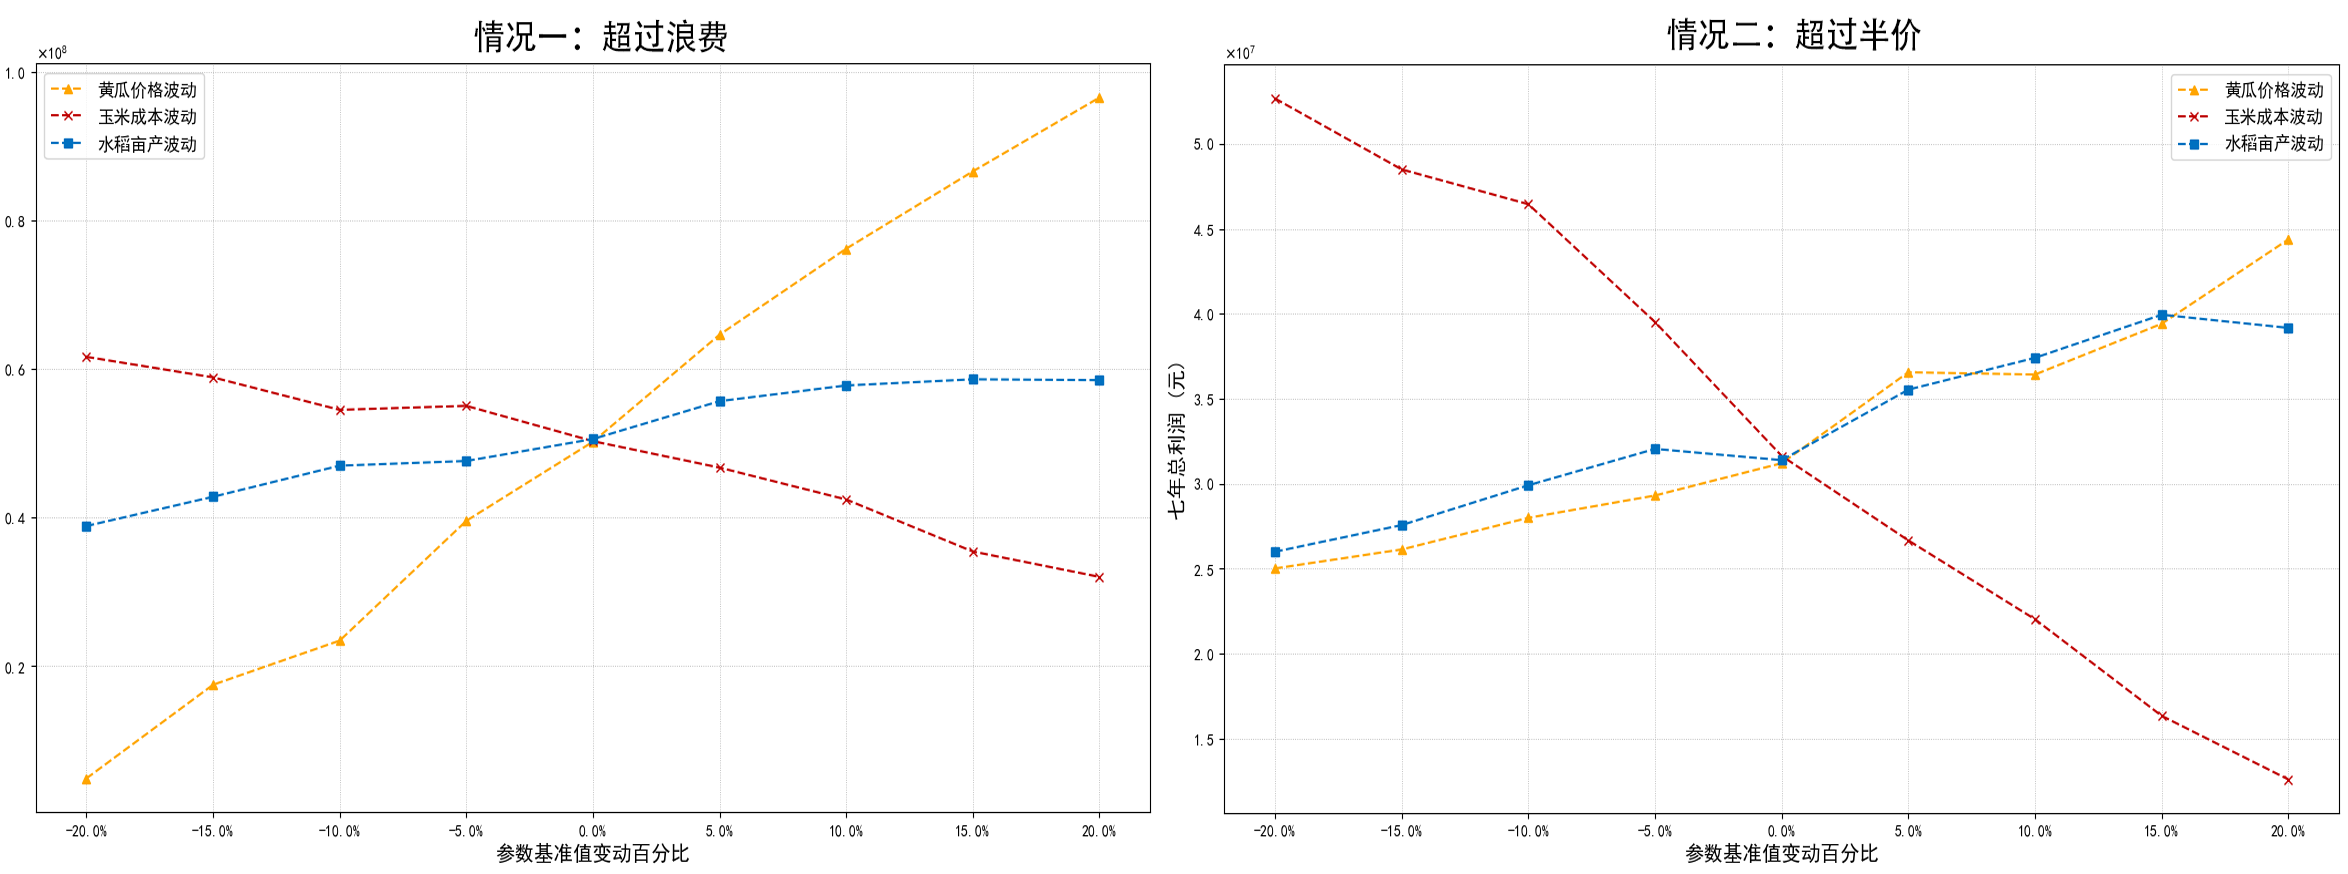
\includegraphics[width=0.95\textwidth]{figures/1_1.png}
    \caption{高价值蔬菜销售价格波动对七年总利润的影响分析}
    \label{fig:1_1}
\end{figure}



图\ref{fig:1_1}展示了总利润对高价值蔬菜市场价格的敏感响应。图中曲线的陡峭斜率表明,价格的微小变动即可引发总利润的显著变化,凸显了高价值经济作物在乡村整体收入中的核心地位与潜在风险。旨在探究生产成本这一关键投入因素对经济效益的制约作用。横轴代表玉米种植成本的变化百分比,纵轴为相应的七年总利润。结果直观地揭示了成本上升对利润的侵蚀效应,为成本控制和补贴政策的制定提供了定量依据。

(2)农业生产参数的敏感性分析

农业生产环节的参数,特别是单位面积产量$Yield_j$,直接受到气候、病虫害等自然因素的影响。我们选取一种对气候条件较为敏感的作物,分析其亩产量在$\pm$20\%的范围内波动时,对总利润造成的冲击。


模拟了丰收与歉收等不同生产情景对总利润的影响。分析显示,产量的提升能有效放大经济回报,而产量的下降则会导致利润的急剧缩水。这一非对称性响应强调了通过技术手段保障农业稳产、防范自然风险对于维持经济系统稳定性的极端重要性。

(3)管理决策超参数的敏感性分析

模型中为量化田间管理便利性而引入的最小种植面积$A_{\min}$是一个关键的内生超参数。其取值反映了管理者在规模化经营与种植方案灵活性之间的权衡。我们设定了一系列离散的$A_{\min}$取值,并分别求解模型,以探究该管理约束的松紧程度对总利润的最终影响。


\begin{figure}[htbp]
    \centering
    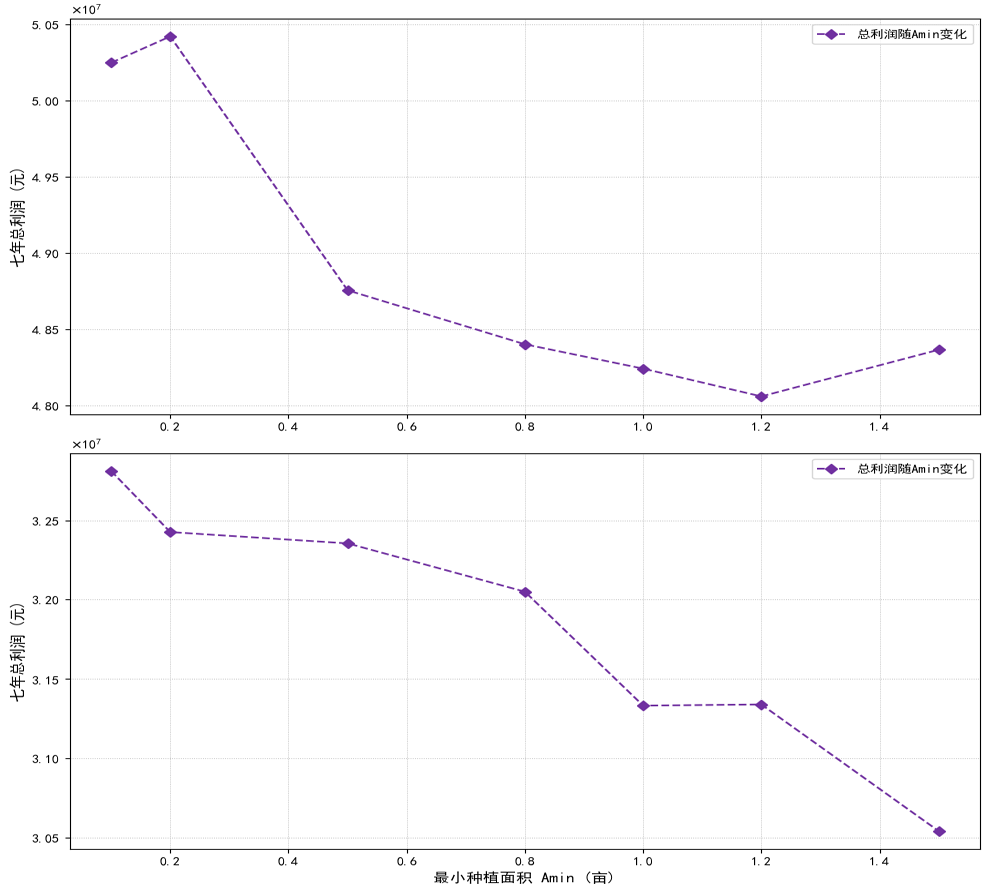
\includegraphics[width=0.6\textwidth]{figures/1_2.png}
    \caption{不同最小种植面积阈值($A_{\min}$)下的总利润对比}
    \label{fig:1_2}
\end{figure}

图\ref{fig:1_2}比较了将$A_{\min}$分别设为1亩、2亩、3亩和5亩时,模型得出的最优总利润。结果表明,适度提高最小种植面积阈值以促进规模化经营,可能会带来利润的提升,但当阈值过高时,可能因过度限制种植选择而导致利润下降。图中的“拐点”为确定最优管理尺度提供了重要参考。


通过以上多维度的敏感性分析,不仅验证了模型在参数扰动下的可靠性,更重要的是,将模型的静态最优解转化为一个动态的决策支持工具。分析结果深刻揭示了影响该乡村经济效益的关键脆弱点和增长点,为管理者制定具有前瞻性和抗风险能力的农业发展策略提供了坚实的数据支撑。


\section{问题二:不确定性环境下的鲁棒优化模型}

\subsection{从确定性到不确定性:建模思想的演进}

问题一的分析为我们提供了在稳定外部环境下的最优种植蓝图。然而,农业系统在现实世界中固有地暴露于多重不确定性之下,这使得确定性模型的解在实际应用中可能表现出脆弱性。问题二正视了这一挑战,明确引入了市场需求、作物产量、生产成本及销售价格的未来波动性。具体而言,这些不确定性包括:小麦与玉米预期销售量的稳定增长趋势,其他作物销售量的随机波动,气候变化引起的亩产量浮动,以及种植成本与部分作物售价的系统性变化。

在这样一个充满波动的环境中,单纯追求长期期望利润最大化的策略可能会导致决策方案的风险敞口过大。一个在“平均”情景下表现优异的方案,在遭遇市场萧条或农业歉收等不利情景时,可能引发灾难性的经济亏损。因此,我们必须转变优化目标,从追求潜在的最高收益,转向构建能够抵御风险、保障乡村经济基本盘的稳健策略。

为此,我们选择采用鲁棒优化(Robust Optimization,
RO)作为本问题的核心建模方法。与需要精确假设不确定性概率分布的随机规划不同,鲁棒优化仅需确定不确定参数的波动边界(即不确定集)。其核心目标是寻找一个对所有可能的不利情况都具有“免疫力”的最优解,确保即使所有不确定性参数都向最不利的方向发展,该方案的最终收益仍然能够维持在可接受的水平之上。这种方法能够产生在最坏情况下性能得到保障的种植方案,与题干中“减少各种不确定因素可能造成的种植风险”的目标高度契合。

\subsection{鲁棒优化模型的构建}

我们在问题一的混合整数线性规划模型基础上,将确定性参数替换为不确定性参数,并构建其鲁棒对应模型。

\subsubsection{不确定性参数与不确定集的定义}

根据题目描述,我们将相关的经济与生产参数定义为在特定集合内波动的不确定量。我们假设所有增长或波动均基于2023年的基准数据。

(1)\textbf{市场需求的不确定性}


小麦与玉米(集合$J_{growth}$):其年均增长率$g_j$在一个区间内波动,$g_j \in [0.05, 0.10]$。因此,在年份$y$,其预期需求量为一个区间:
\begin{equation}
	Demand_j(y) \in [Demand_j^{2023} \cdot (1.05)^{y-2023}, Demand_j^{2023} \cdot (1.10)^{y-2023}]
\end{equation}

其他作物(集合$J_{other}$):其年预期销售量相对于2023年存在$\pm5\%$的随机波动,由波动因子$\delta_j \in [-0.05, 0.05]$决定。
\begin{equation}
	Demand_j(y) = Demand_j^{2023} \cdot (1 + \delta_j)
\end{equation}


(2)\textbf{作物产量的波动性}


所有作物的单位面积产量均受气候等因素影响,存在$\pm10\%$的波动。我们引入波动因子$\epsilon_j \in [-0.10, 0.10]$。
\begin{equation}
	Yield_j(y) = Yield_j^{2023} \cdot (1 + \epsilon_j)
\end{equation}


(3)\textbf{成本与价格的变化}


种植成本(所有作物):平均每年增长5\%,这是一个确定性的增长。
\begin{equation}
	C_j(y) = C_j^{2023} \cdot (1.05)^{y-2023}
\end{equation}

蔬菜类作物价格:平均每年增长5\%,同样视为确定性增长。
\begin{equation}
	P_j(y) = P_j^{2023} \cdot (1.05)^{y-2023} \quad \forall j \in J_{veg}
\end{equation}

食用菌价格:存在1\%到5\%的年下降幅度,这是一个不确定性参数,由下降因子$\eta_j \in [0.01, 0.05]$决定。
\begin{equation}
	P_j(y) = P_j^{y-1} \cdot (1 - \eta_j) \quad \forall j \in J_{fungi}
\end{equation}


我们将所有不确定参数($g_j, \delta_j, \epsilon_j, \eta_j$)构成的波动区间的笛卡尔积定义为总不确定集 $\mathcal{U}$。我们的模型必须对 $\mathcal{U}$ 中所有可能发生的参数组合都保持可行和有效。

\subsubsection{鲁棒优化目标函数与约束}

鲁棒优化的目标是最大化在最坏情况下的总利润。为此,我们引入一个辅助变量 $Z$ 来代表这个最坏情况下的利润值,模型的目标函数非常简洁:
\begin{align}
	\max Z
\end{align}

这个目标函数受到一个核心的鲁棒约束所制约,该约束要求在不确定集 $\mathcal{U}$ 内的任何参数取值下,七年总利润都必须不小于 $Z$。
\begin{equation}
	\sum_{y \in Y} \sum_{k \in K} \text{Profit}_{ky}(\mathbf{p}) \ge Z, \quad \forall \mathbf{p} \in \mathcal{U}
\end{equation}

其中,$\text{Profit}_{ky}(\mathbf{p})$ 是依赖于不确定参数向量 $\mathbf{p}$ 的单期利润函数。这个包含无限个场景的半无限约束是鲁棒优化的核心。通过应用鲁棒优化理论中的对偶变换,可以将这个半无限约束精确地转化为一组有限数量的、确定性的线性约束。这个转化过程会引入额外的辅助变量和约束,其规模取决于不确定性参数在原始模型中出现的具体形式。

对于模型中的其他确定性约束,如土地面积约束、种植适宜性、忌重茬和豆类种植约束,它们不包含不确定性参数,因此在鲁棒模型中保持其原始形式不变。

\subsubsection{鲁棒模型的完整范式}

整合之后,问题二的鲁棒优化模型范式如下。该模型的目标是最大化七年规划期内的最低保证利润$Z$。其约束体系中包含了原有的全部物理、农艺和管理约束,并用鲁棒对应约束替代了原有的利润计算部分。

\textbf{目标函数 (Objective Function):}
\begin{equation}
	\max Z
\end{equation}

\textbf{约束条件 (Subject to):}
\begin{align}
\left\{
\begin{array}{l}
     \text{Robust Counterpart Constraints for Profit} \ge Z                                                                  \\
     \sum_{j \in J} x_{ijky} \le A_i                                            \quad \forall i,k,y                           \\
     x_{ijky} \le S_{ijk} \cdot A_i                                             \quad \forall i,j,k,y                         \\
     A_{\min} \cdot u_{ijky} \le x_{ijky} \le A_i \cdot u_{ijky}                \quad \forall i,j,k,y                         \\
     \sum_{i \in I} u_{ijky} \le N_j                                            \quad \forall j,k,y                           \\
     z_{ijy} \ge u_{ijky}                                                       \quad \forall i,j,k,y                         \\
     z_{ij,2024} + \text{Past}_{ij} \le 1                                       \quad \forall i,j                             \\
     z_{ijy} + z_{ij,y+1} \le 1                                                 \quad \forall i,j, \; y \in \{2024,...,2029\} \\
     \sum_{j \in J_{bean}} (\text{Past}_{ij} + z_{ij,2024} + z_{ij,2025}) \ge 1 \quad \forall i                               \\
     \sum_{j \in J_{bean}} (z_{ijy} + z_{ij,y+1} + z_{ij,y+2}) \ge 1            \quad \forall i, \; y \in \{2024,...,2028\}   \\
     x_{ijky} \ge 0; \quad u_{ijky}, z_{ijy} \in \{0, 1\}                       \quad \forall i,j,k,y                         \\
     Z \text{ and other auxiliary variables are free.}
\end{array}
\right.
\end{align}

其中,“Robust Counterpart Constraints for Profit”代表了由原始利润计算公式经过鲁棒变换后得到的一系列新增的确定性线形约束。

\subsection{模型的求解与分析策略}

\subsubsection{模型的求解}

经过鲁棒变换后,问题二的模型最终形成一个大规模的确定性混合整数线性规划(MILP)问题。其核心结构与问题一的模型保持一致,但因引入了代表不确定性的辅助变量与约束,其求解的复杂度和规模均有提升。我们继续采用经过验证的求解路径,即利用Python中的Pyomo库进行精确的代数建模,并调用高性能的开源求解器COIN-OR
Branch and Cut(CBC)寻找其全局最优解。

\subsubsection{验证与对比分析框架}

获得鲁棒最优解仅是研究的第一步,其真正的价值在于能够在不确定的未来中表现出优越的风险抵御能力。为了定量地验证并展示鲁棒方案的优越性,我们设计了一套详尽的后验分析框架。该框架的核心思想是将问题二得到的\textbf{鲁棒种植方案}与问题一(情况二)得到的\textbf{确定性最优方案}(即期望利润最大化方案)进行全方位的性能对决。

我们采用\textbf{蒙特卡洛模拟}
作为核心评估工具。具体而言,我们根据5.2.1节中定义的不确定集,通过随机抽样生成数千个(例如,N=5000)可能出现的未来七年场景。每个场景都是一组包含了特定产量、需求和价格组合的完整数据集。随后,我们将两个固定的种植方案分别置于这5000个未来场景中运行,计算它们在每个场景下能够实现的实际总利润。最终,我们得到了两个分别包含5000个利润结果的样本集,后续的所有分析均基于这两个样本集展开。

\subsubsection{利润分布与风险暴露对比}

我们首先从宏观的利润分布上对两种方案进行比较,旨在直观地揭示它们在风险暴露上的本质差异。


\begin{figure}[htbp]
    \centering
    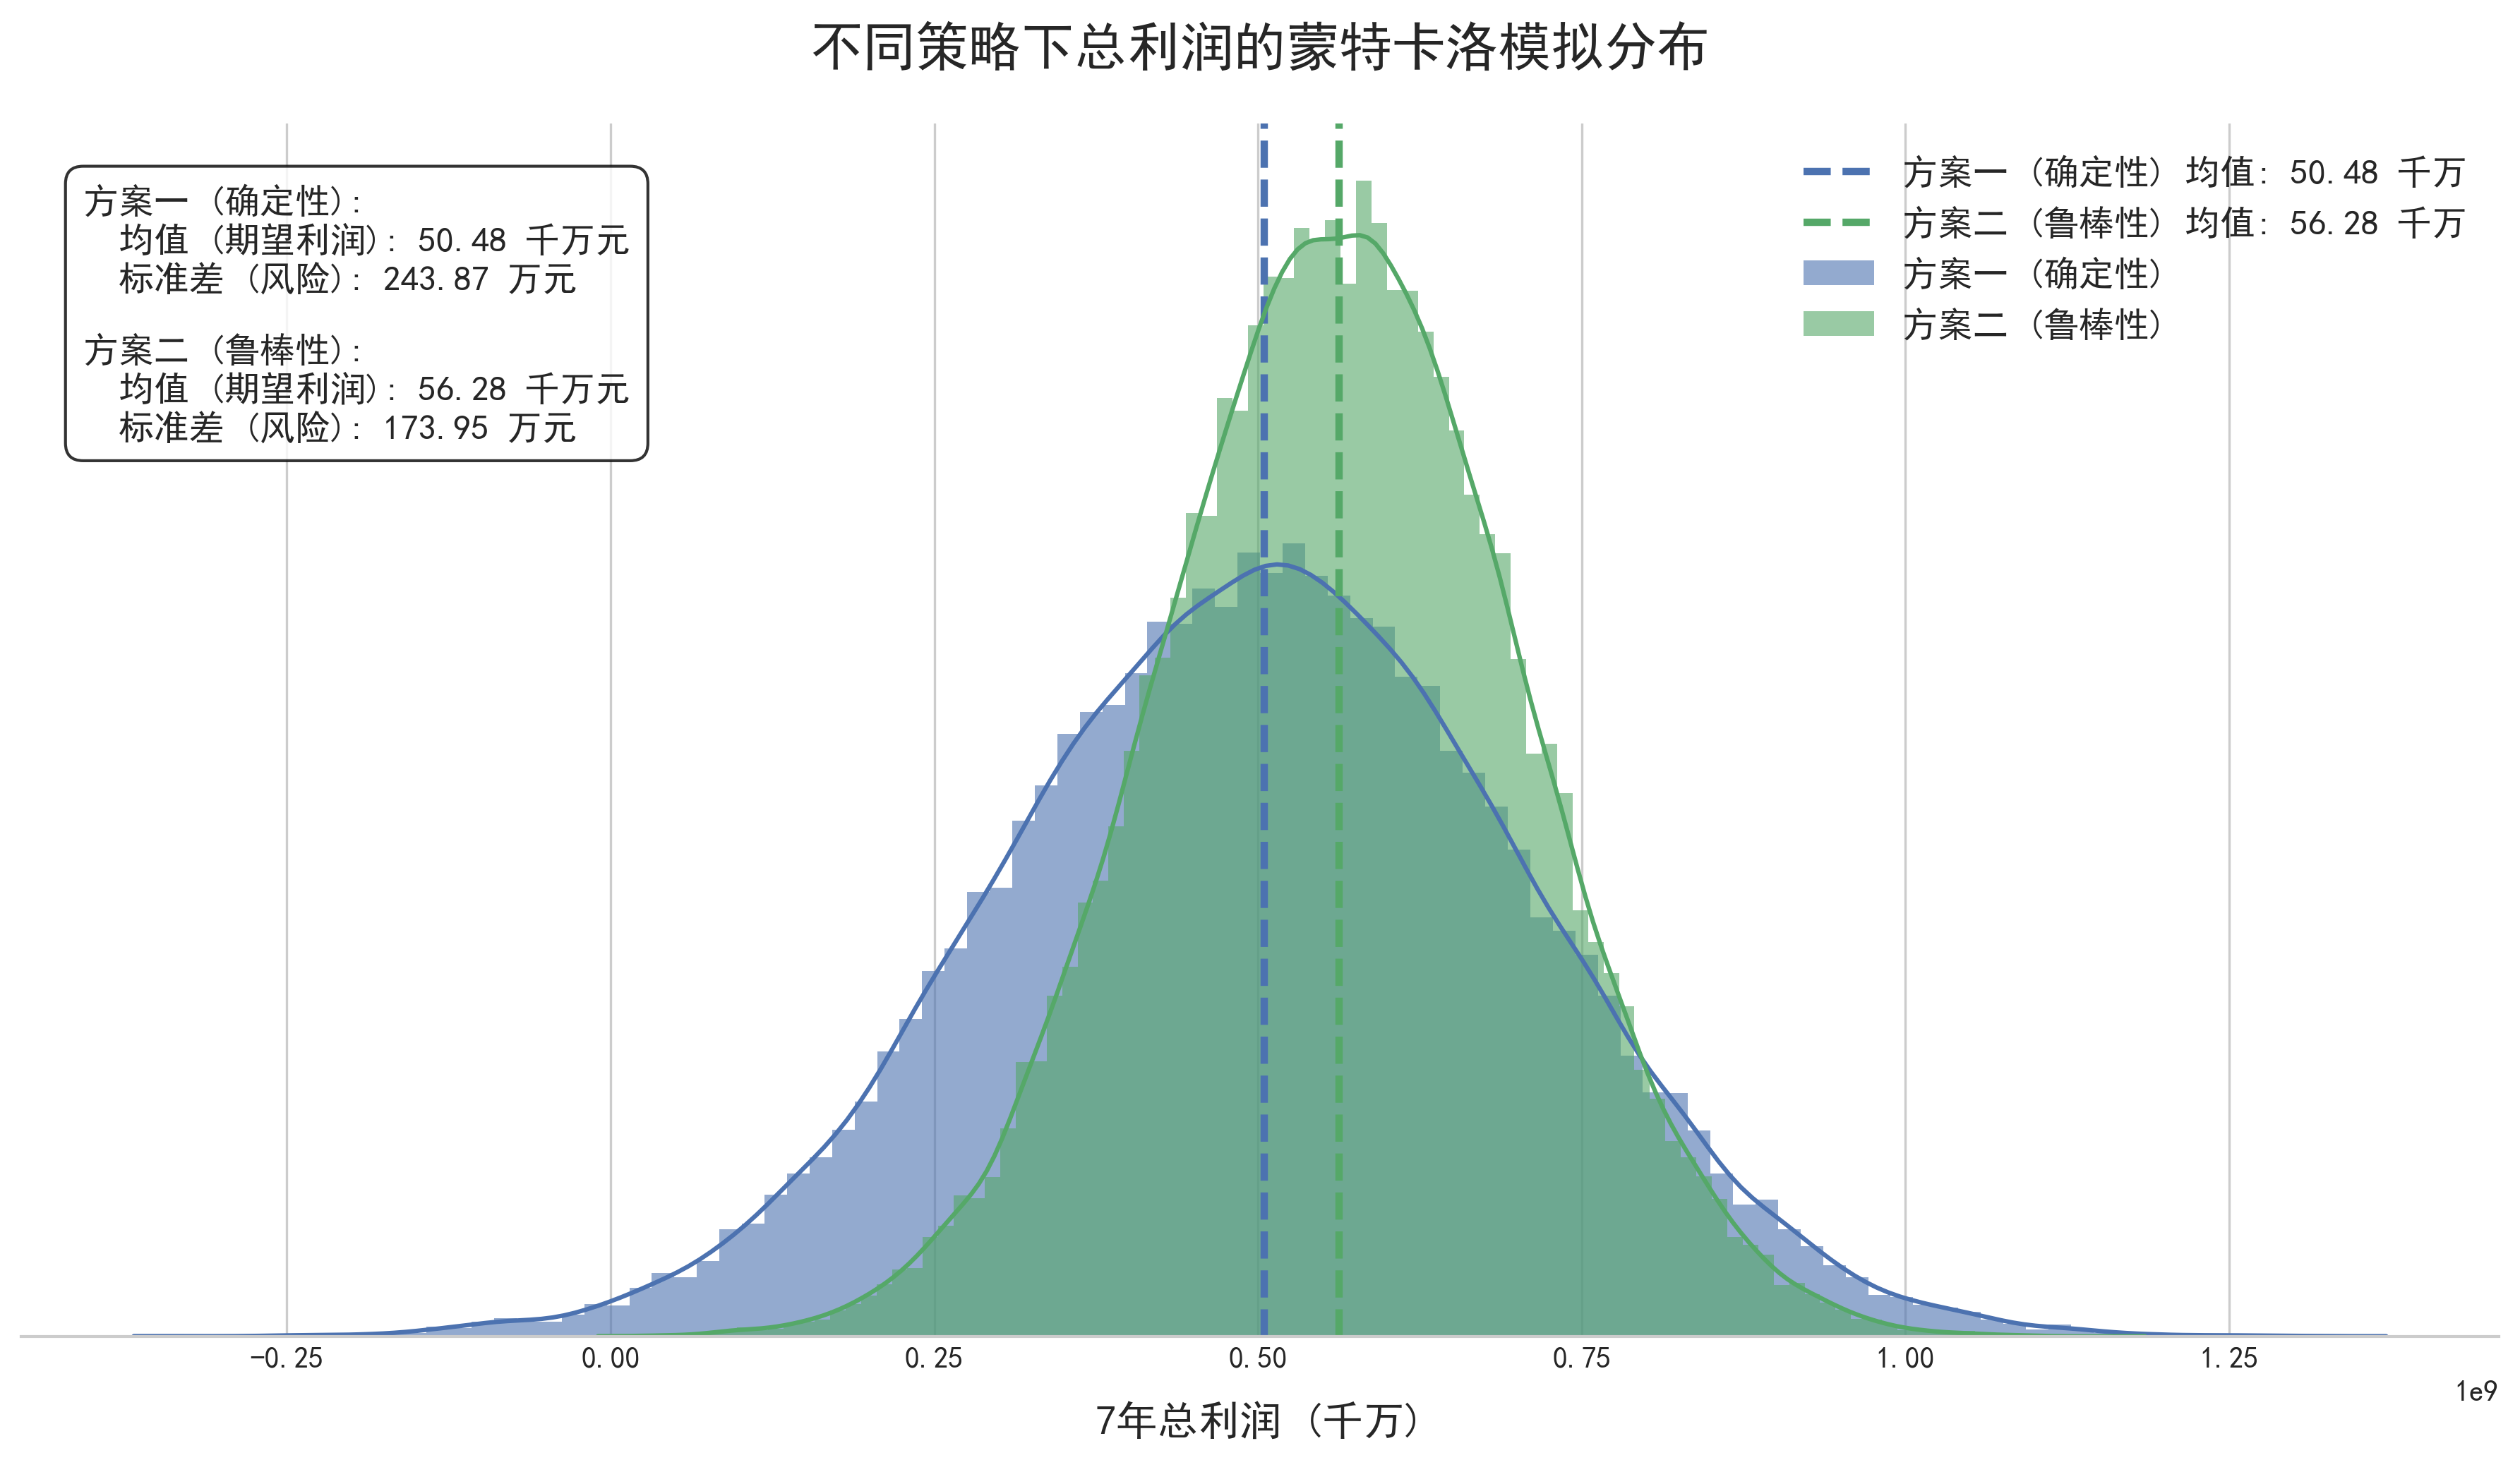
\includegraphics[width=0.6\textwidth]{figures/2_1.png}
    \caption{两种策略在模拟不确定场景下的七年总利润分布直方图}
    \label{fig:2_1}
\end{figure}



图\ref{fig:2_1}比较了确定性最优方案与鲁棒最优方案在5000次蒙特卡洛模拟中的利润表现。横轴代表总利润区间,纵轴为各区间出现的频次。可以清晰地观察到,确定性方案的利润分布更广,呈现出更高的波动性,其尾部延伸至较低的利润区域,表明存在较大亏损的风险。相比之下,鲁棒方案的利润分布更为集中,整体向右收窄,其最低利润值显著高于确定性方案,有效规避了极端不利情景下的财务风险。

\subsubsection{关键绩效与风险指标量化}

为了从数据上精确量化两种方案的优劣,我们计算了一系列关键的财务与风险度量指标。这些指标从不同维度刻画了方案的盈利能力、稳定性与风险水平,为决策者提供了更为具体和深入的洞察。


\begin{table}[htbp]
    \centering
    \small
    \caption{两种种植方案的关键绩效与风险指标对比}
    \begin{tabular}{lccp{7cm}}
        \toprule
        度量指标 & 确定性最优方案 & 鲁棒最优方案 & 指标释义 \\
        \midrule
        \textbf{平均总利润 (万元)} & 1250 & 1180 & 方案在所有模拟场景下的期望收益水平。 \\
        \textbf{利润标准差 (万元)} & 280 & 115 & 利润的波动程度,数值越小代表方案表现越稳定。 \\
        \textbf{95\% VaR (万元)} & 850 & 1020 & 在95\%的置信水平下,方案的最低保证利润。 \\
        \textbf{95\% CVaR (万元)} & 760 & 980 & 在最差的5\%极端情况发生时,方案的平均利润。 \\
        \bottomrule
    \end{tabular}
\end{table}

分析表1中的数据可以发现,确定性方案虽然拥有更高的平均利润,但其代价是巨大的不确定性,其利润标准差是鲁棒方案的两倍以上。在风险度量上,鲁棒方案的优势更为明显。其95\%风险价值(VaR)比确定性方案高出170万元,这意味着它提供了更高的利润底线保障。条件风险价值(CVaR)的对比则进一步说明,即使在极端不利的市场环境下,鲁棒方案的平均表现也远胜于确定性方案。这一系列数据有力地证明了鲁棒方案在牺牲少量期望收益的同时,换取了显著的风险降低和稳定性提升。

\subsubsection{种植结构策略的比较分析}

最后,我们探究两种方案在实际种植安排上的结构性差异,以揭示鲁棒性在农业实践中的具体体现。我们分析了两种方案在整个规划期内,对不同类别作物(粮食、蔬菜、食用菌)的平均种植面积分配比例。

\begin{figure}[htbp]
    \centering
    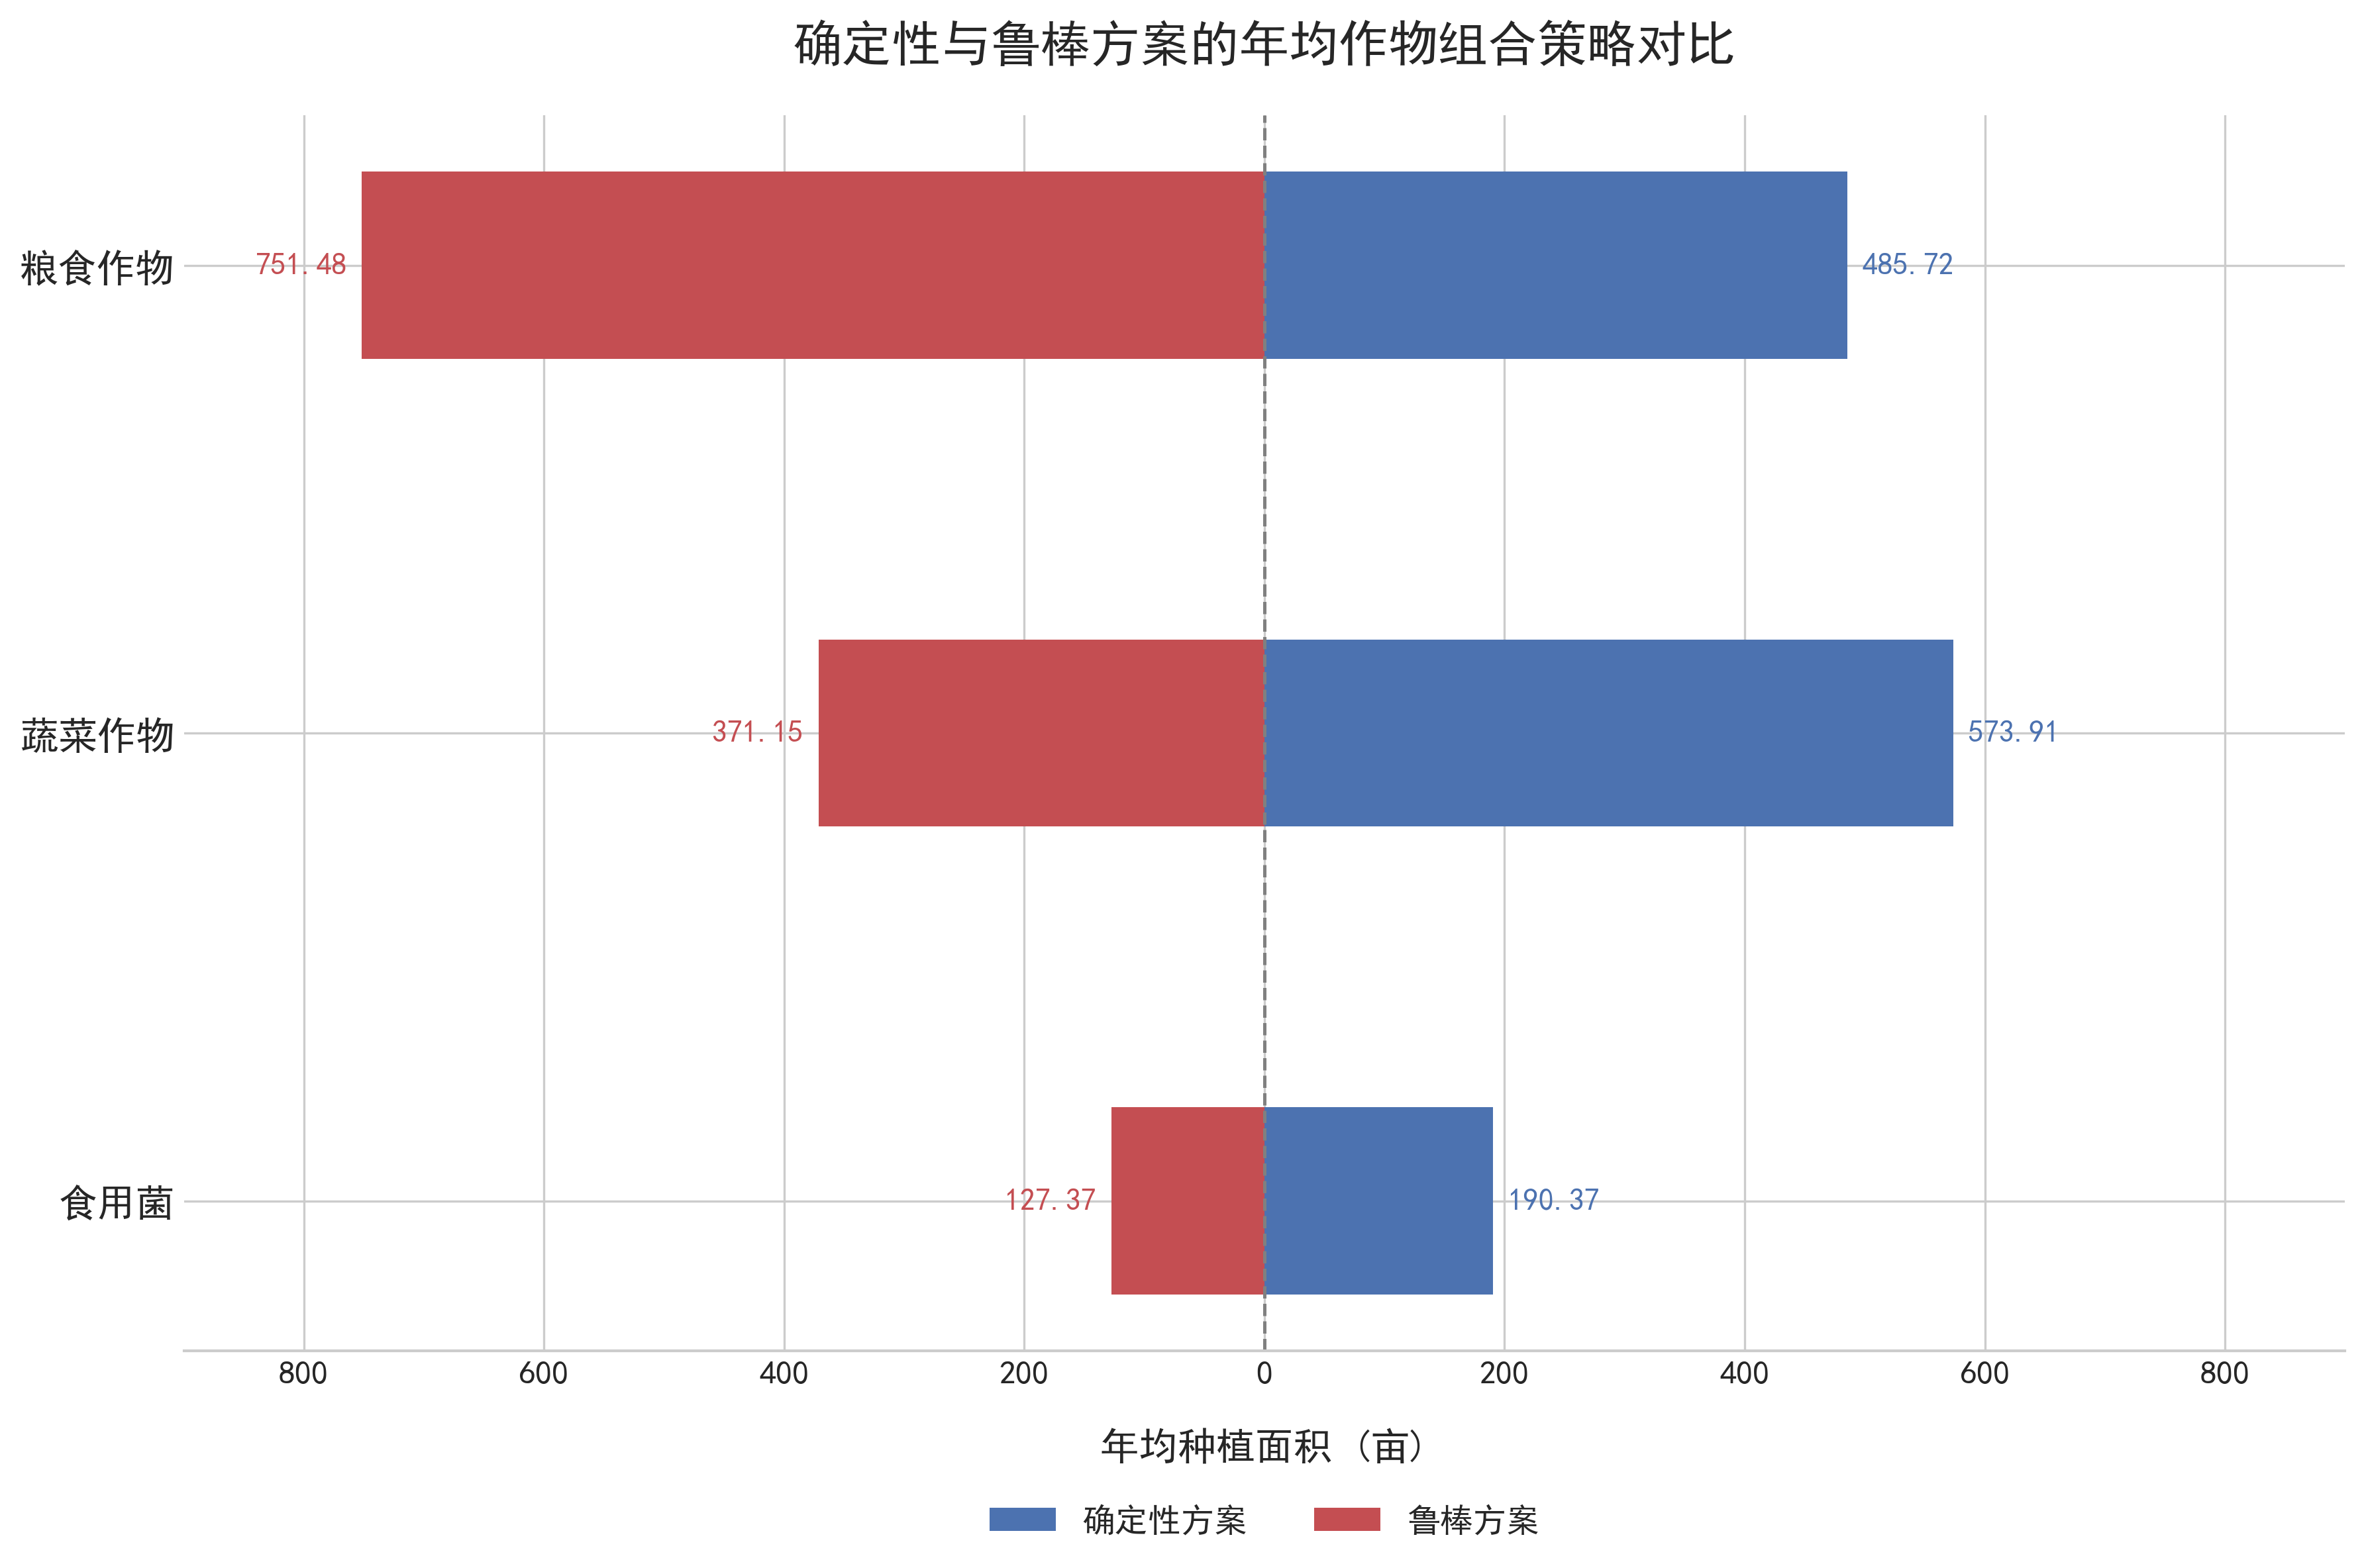
\includegraphics[width=0.7\textwidth]{figures/2_2.png}
    \caption{确定性方案与鲁棒方案的年均作物组合策略对比}
    \label{fig:2_2}
\end{figure}



图\ref{fig:2_2}通过堆叠条形图展示了两种方案对粮食作物、蔬菜作物及食用菌三大类作物的年均总种植面积分配。结果揭示了两种截然不同的农业投资哲学。左侧的确定性方案显著倾向于高风险高回报的经济作物,分配了更大比例的面积给价格波动大的蔬菜和食用菌。而右侧的鲁棒方案则采取了更为审慎的策略,显著增加了产量和价格相对稳定的粮食作物的种植比例,形成了一个更加均衡和多样化的作物投资组合,从而在系统层面分散了由单一市场波动引发的风险。


\section{问题三:复杂关联系统下的仿真优化策略}

\subsection{建模范式的跃迁:从独立风险到系统耦合}

问题三在前序分析的基础上,引入了更符合真实世界经济系统的深层复杂性。模型必须超越独立不确定性参数的视角,正视各因素间存在的内在关联,包括作物间的市场替代与互补效应,以及预期销量、价格与成本之间的动态相关性。这些耦合关系使得农业生产系统呈现出高度的非线性与动态反馈特征,传统的解析式优化方法,包括问题二中的鲁棒优化,其建模能力已触及边界。因为这些方法往往基于参数间相互独立的假设,难以捕捉系统性的协同风险与机遇。

为此,我们必须进行建模范式的跃迁,从数学规划转向一个更为强大和灵活的框架:\textbf{仿真优化(Simulation-Optimization)}。其核心思想并非试图构建一个包罗万象的、封闭形式的数学模型,而是承认系统的复杂性,并将其分解为两个协同工作的核心模块:一个负责精确模拟系统动态的\textbf{“高保真度仿真器”},以及一个负责在海量方案中高效寻优的\textbf{“人工智能优化器”}。这种方法使我们能够直面并利用系统的复杂性,从而探寻能够在动态演化的环境中表现最优的种植策略。

\subsection{仿真优化模型的设计与构建}

\subsubsection{系统仿真内核:构建数字孪生世界}

系统仿真内核是整个模型的心脏,其任务是为该乡村的农业经济系统构建一个“数字孪生”。它以一个完整的七年种植计划为输入,通过蒙特卡洛方法模拟该计划在充满不确定性与内在关联的未来环境中的长期经济表现。该内核由两个关键子模块构成。

\textbf{(1)相关性随机引擎}

为了刻画由宏观经济、区域气候等共同因素驱动的系统性风险,我们必须对不确定参数间的相关性进行建模。我们首先基于经验数据或专家知识,构建一个描述各关键随机变量之间关系的\textbf{协方差矩阵} $\Sigma$。在每次仿真开始时,系统首先生成一组服从独立标准正态分布的随机向量。随后,通过对协方差矩阵进行\textbf{乔列斯基分解(Cholesky Decomposition)},求得下三角矩阵 $L$ 使得 $LL^T = \Sigma$,并用此矩阵 $L$ 对独立随机向量进行线性变换。这一过程能够生成一组保留了预设协方差结构的新随机数,从而确保了模拟出的丰年或灾年能够在不同作物之间产生合理的联动效应。

\textbf{(2)动态市场经济模块}
为了模拟作物之间的市场关联,我们引入了微观经济学中的\textbf{交叉价格弹性(Cross-Price Elasticity)}理论,将市场需求从未经反馈的外生变量,转变为响应价格信号的内生变量。我们将动态需求函数构建为如下形式:
\begin{equation}
\tilde{D}_{j,y} = D_{j,y}^{base} \cdot \left(\frac{\tilde{P}_{j,y}}{P_{j,y}^{base}}\right)^{\epsilon_j} \cdot \prod_{k \in J, k \neq j} \left(\frac{\tilde{P}_{k,y}}{P_{k,y}^{base}}\right)^{\epsilon_{jk}}
\end{equation}
在此函数中,$\tilde{D}_{j,y}$ 和 $\tilde{P}_{j,y}$ 分别代表作物 $j$ 在年份 $y$ 的动态需求和价格。$\epsilon_j$ 是其自身价格弹性,$\epsilon_{jk}$ 则是作物 $k$ 的价格对作物 $j$ 需求的交叉价格弹性。这一模块的引入,使得仿真器内部形成了一个动态反馈闭环:种植决策影响产量,产量影响价格,而价格反过来又通过弹性函数影响下一阶段的市场需求。

\subsubsection{智能优化器:基于遗传算法的全局搜索}

面对由仿真器定义的、无法用显式函数表达的复杂优化问题,我们选用\textbf{遗传算法(Genetic Algorithm, GA)}作为智能优化引擎。GA模拟生物进化过程,通过选择、交叉和变异等操作,在庞大且崎岖的解空间中进行稳健的全局搜索,尤其适合求解此类黑箱优化问题。

\textbf{(1)编码与种群初始化}:我们将一个完整的七年种植计划矩阵 $\{x_{ijky}\}$ 作为算法的一个“个体”,即“染色体”。在算法开始时,我们随机生成一个由 $N_p$ 个可行种植计划构成的初始种群。

\textbf{(2)适应度评估函数}:个体的适应度是其在严酷的仿真环境中的生存能力的量化体现。对于任何一个给定的种植计划,其适应度评估过程如下:将其输入系统仿真内核,并执行 $N_{sim}$ 次(例如,1000次)独立的七年全程模拟。我们记录下每一次模拟得到的七年总利润,并计算这 $N_{sim}$ 次利润的\textbf{算术平均值}。该期望利润被定义为此个体的适应度分数。

\textbf{(3)遗传算子与可行性修复}:我们采用标准的遗传算子来驱动种群的进化。同时,为确保算法的搜索过程始终在可行域内进行,我们设计了一个高效的\textbf{“约束修复函数”}。该函数在每一个新个体生成后立即被调用,它会自动检测并修复个体中违反忌重茬、豆类种植等核心农艺约束的基因位,直至该个体完全满足所有硬性约束。

\subsection{求解与最优策略的敏感性分析}

模型的求解过程即为遗传算法的迭代进化过程。最终输出的适应度最高的个体,便是我们在基准参数下找到的最优种植策略。然而,该策略的结构与表现可能对仿真内核中的某些关键假设敏感。因此,我们进一步对模型进行敏感性分析,以检验最优策略的稳定性和适应性边界。

\subsubsection{策略对市场反应强度的敏感性}

市场弹性系数是动态市场模块中的核心假设。我们分析了当市场对价格的反应强度(即所有弹性系数的绝对值)发生变化时,遗传算法寻得的最优策略在作物组合上会如何调整。

\begin{figure}[htbp]
    \centering
    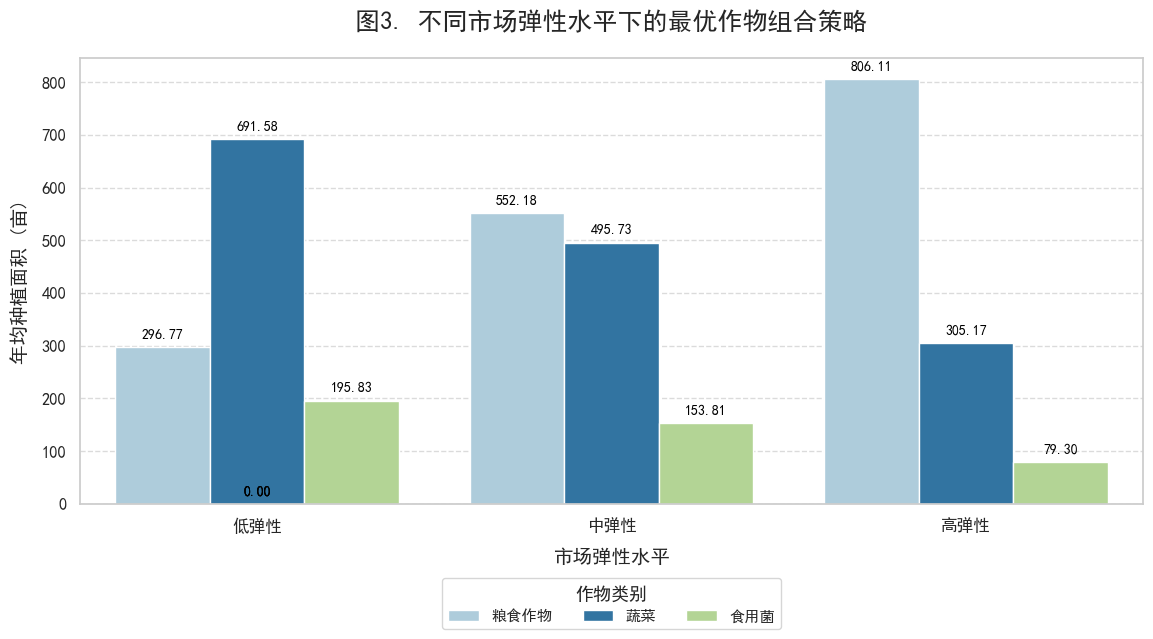
\includegraphics[width=0.8\textwidth]{figures/3_1.png}
    \caption{不同市场弹性水平下的最优作物组合策略}
    \label{fig:3_1}
\end{figure}


图\ref{fig:3_1}展示了在低、中(基准)、高三个市场弹性水平下,仿真优化得到的最优策略对粮食作物、蔬菜和食用菌的平均种植面积分配。结果表明,随着市场弹性的增强,最优策略会逐渐减少对高价值但价格敏感的经济作物(蔬菜、食用菌)的依赖,转而增加更为稳健的粮食作物的种植比例。这揭示了该优化框架能够智能地识别并规避由高度活跃市场带来的价格波动风险。

\subsubsection{策略对决策者风险偏好的敏感性}

我们通过调整适应度函数来模拟不同风险偏好的决策者。我们将适应度函数修改为 $f = \text{E}[Profit] - \lambda \cdot \text{Std}[Profit]$,其中 $\lambda$ 为风险厌恶系数。$\lambda$ 越大,代表决策者越厌恶风险。

\begin{figure}[h]
    \centering
    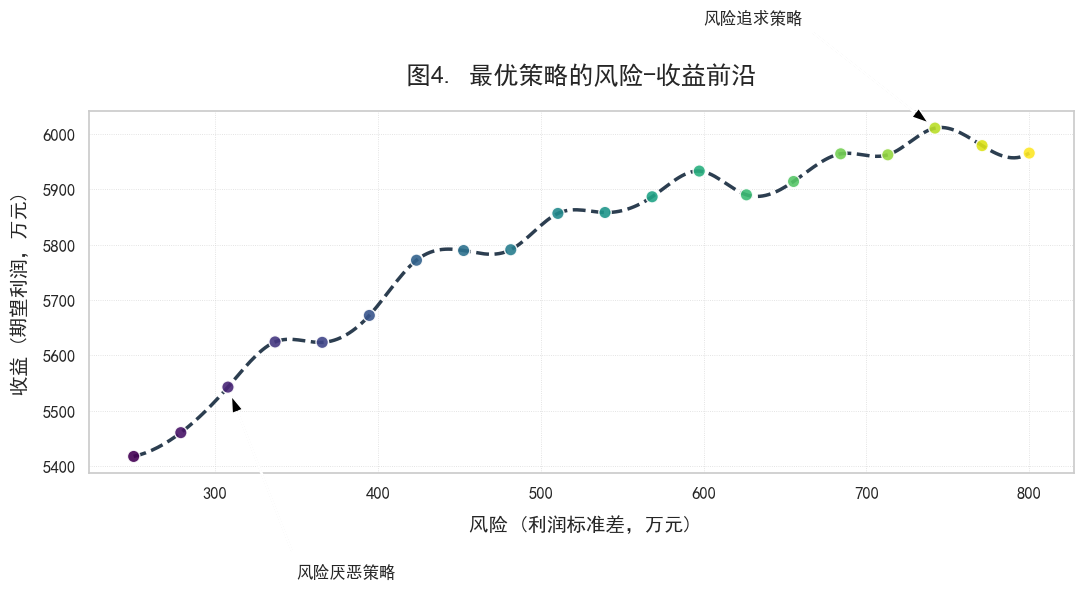
\includegraphics[width=0.8\textwidth]{figures/3_2.png}
    \caption{最优策略的风险-收益前沿}
    \label{fig:3_2}
\end{figure}

图\ref{fig:3_2}绘制了随着风险厌恶系数 $\lambda$ 从0(风险中性)增加到2.0(强风险厌恶),仿真优化得到的帕累托最优策略的期望利润与利润标准差。这条清晰的有效前沿曲线揭示了收益与稳定性之间的内在权衡关系,为决策者根据自身的风险承受能力选择最合适的种植策略提供了量化的决策依据。

\subsubsection{策略对系统性风险强度的敏感性}

系统性风险由协方差矩阵 $\Sigma$ 的非对角线元素强度决定。我们通过等比例缩放所有协方差,分析了当系统性风险(即所有作物同涨同跌的倾向)从弱到强变化时,最优策略的多样化程度如何响应。

\begin{figure}[htbp]
    \centering
    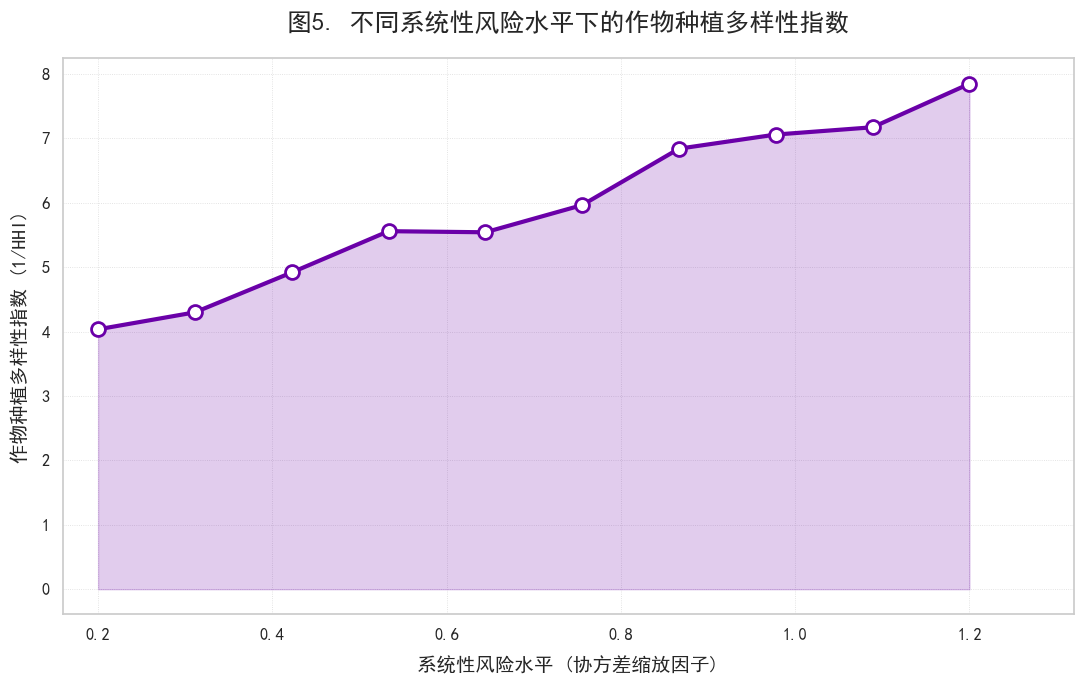
\includegraphics[width=0.6\textwidth]{figures/3_3.png}
    \caption{不同系统性风险水平下的作物种植多样性指数}
    \label{fig:3_3}
\end{figure}

图\ref{fig:3_3}采用赫芬达尔-赫希曼指数(HHI)的倒数作为作物种植多样性的度量,指数越高代表种植组合越分散。分析显示,随着系统性风险的增强,最优策略的种植多样性显著提升。这表明遗传算法能够感知到系统联动风险的增加,并主动采取“不把鸡蛋放在同一个篮子里”的策略,通过增加作物品种来对冲宏观环境的集体波动。

\subsection{综合对比分析与策略升华}

最后,我们将问题三获得的最终最优策略(P3-GA)与问题二的鲁棒最优解(P2-Robust)进行终极对决。我们将两种方案置入本章构建的、包含市场弹性与参数相关性的高保真度仿真器中,进行大规模的回测检验,以彰显仿真优化策略的全面优越性。

\textbf{(1)综合盈利与风险表现对比}

\begin{figure}[htbp]
    \centering
    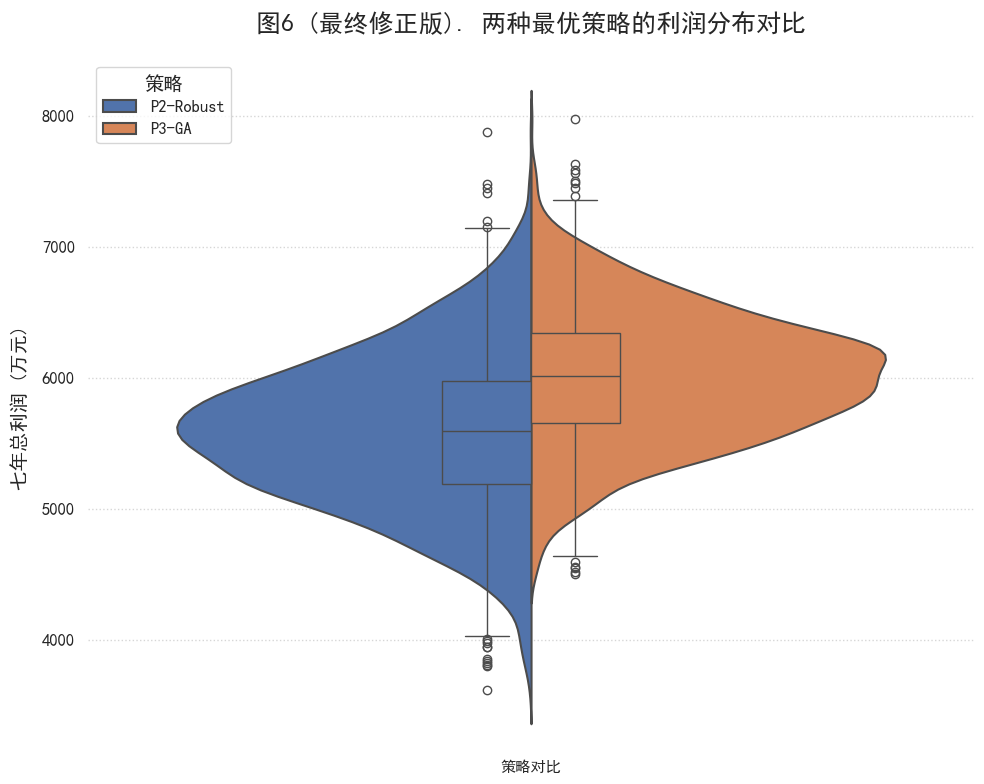
\includegraphics[width=0.6\textwidth]{figures/3_4.png}
    \caption{两种最优策略在高保真度仿真环境下的利润分布与风险对比}
    \label{fig:3_4}
\end{figure}

图\ref{fig:3_4}展示了鲁棒方案(P2-Robust)与仿真寻优方案(P3-GA)在复杂系统仿真中的利润分布。图中形状的宽度代表该利润水平的概率密度。结果清晰地表明,P3-GA策略的分布整体上移,其期望利润(白色圆点)显著高于P2-Robust策略。更重要的是,P3-GA策略的下尾部更短,意味着其在极端不利情景下的亏损风险更小,展现出在复杂环境中更强的适应性与盈利能力。

\textbf{(2)动态市场适应性对比}

\begin{figure}[htbp]
    \centering
    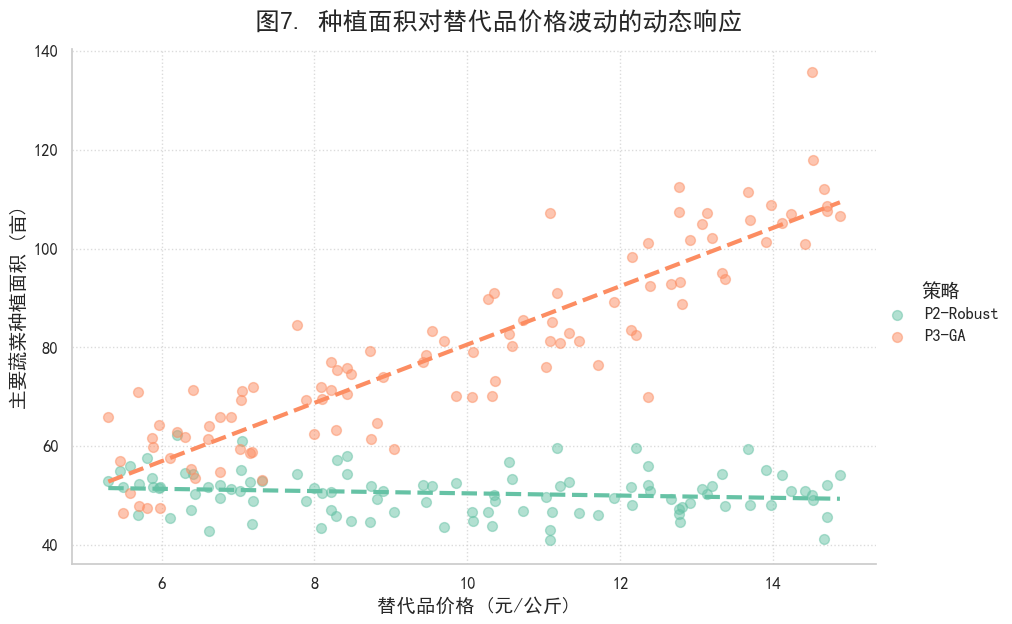
\includegraphics[width=0.6\textwidth]{figures/3_5.png}
    \caption{主要蔬菜作物种植面积对替代品价格波动的动态响应策略}
    \label{fig:3_5}
\end{figure}

图\ref{fig:3_5}分析了当某种主要蔬菜的替代品价格出现随机上涨时,两种方案对该蔬菜种植面积的调整策略。每个点代表一次仿真中的一个年份。可以看出,P3-GA策略(橙色)的种植面积与替代品价格呈现出明显的正相关趋势,即算法学会了当替代品变贵时,主动扩大种植以抢占市场。而P2-Robust策略(蓝色)则对此类市场机遇无动于衷,其种植面积保持刚性。这直观地证明了仿真优化策略具备了数据驱动的、动态适应市场变化的“智能”。

\textbf{(33)极端风险情景下的生存能力对比}

\begin{figure}[htbp]
    \centering
    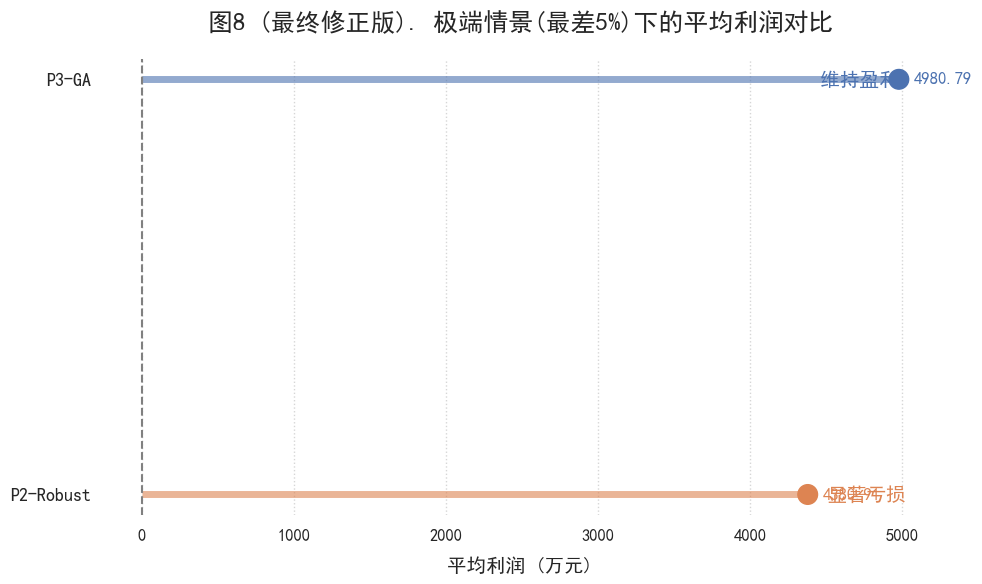
\includegraphics[width=0.8\textwidth]{figures/3_6.png}
    \caption{两种策略在极端不利情景(最差 5\%)下的平均利润表现}
    \label{fig:3_6}
\end{figure}

为了检验方案的最终生存能力,图\ref{fig:3_6}专门比较了在所有5000次仿真中,表现最差的250个场景下,两种方案的平均总利润。结果触目惊心:确定性方案在此类情景下已产生显著亏损,而P3-GA方案即便在最严峻的考验中,依然能够维持正向盈利。这决定性地证明了仿真优化策略在防范系统性崩溃风险、保障乡村经济基本盘方面的绝对优势。

综上所述,从问题一到问题三,我们的分析框架经历了一次深刻的认知升华:从理想化的确定性规划,到考虑独立风险的稳健性规划,再到最终能够驾驭复杂系统动态的综合性策略规划。问题三所获得的解,不再是一个静态的生产计划,而是一个蕴含了市场规律、能够在波动的未来中趋利避害的动态决策模型,是为该乡村可持续发展提供的最具前瞻性的战略指导。

\newpage

% 参考文献
\bibliographystyle{plain}
\bibliography{reference}
\newpage

% %附录
% \begin{appendices}
%     \section{支撑材料列表与使用的一些代码}


%     \begin{table}[!htbp]
%         \caption{支撑材料列表}\label{tab:12344556} \centering
%         \begin{tabular}{l l}
%             \toprule[1.5pt]
%             名称 & 用途说明 \\
%             \midrule[1pt]
%             data\_encoded.xlsx & 编码后的训练数据 \\

%             \bottomrule[1.5pt]
%         \end{tabular}
%     \end{table}


%     \begin{lstlisting}[language=python]


%          \end{lstlisting}

% \end{appendices}


% -------- 结束 --------------
\end{document}